% This file is part of the causal-kepler project
% Copyright 2013, 2014 the authors.

% # to-do
% - write causal description

\documentclass[12pt, preprint]{aastex}

\usepackage{graphicx}
\usepackage{caption} 
\usepackage{subcaption} 

\usepackage{hyperref}
\usepackage{url}

\usepackage{natbib}

\graphicspath{{figures/}}

\newcommand{\notenglish}[1]{\textit{#1}}
\newcommand{\sic}{\notenglish{sic}}
\newcommand{\project}[1]{\textsl{#1}}
\newcommand{\Kepler}{\project{Kepler}}
\newcommand{\name}{CPM}
\newcommand{\set}[1]{\mathcal{#1}}
\newcommand{\given}{\,|\,}
\newcommand{\todo}[1]{\textbf{#1}}

\newcommand{\Bernhard}[1]{$\bullet$\footnote{{\bf Bernhard:} #1}}
\newcommand{\Dun}[1]{$\bullet$\footnote{{\bf Dun:} #1}}


\begin{document}

\title{
  Calibrating the pixel-level Kepler imaging data with a causal data-driven model
 \\ 
}
\author{%
  Dun~Wang\altaffilmark{\ref{CCPP}},
  Dan~Foreman-Mackey\altaffilmark{\ref{CCPP}},
  David~W.~Hogg\altaffilmark{\ref{CCPP},\ref{CDS},\ref{MPIA},\ref{email}},
  Bernhard~Sch\"olkopf\altaffilmark{\ref{MPIIS}},
  others%
}
\newcounter{address}
\setcounter{address}{1}
\altaffiltext{\theaddress}{\stepcounter{address}\label{CCPP}%
  Center for Cosmology and Particle Physics, Department of Physics, New York University}
\altaffiltext{\theaddress}{\stepcounter{address}\label{CDS}%
  Center for Data Science, New York University}
\altaffiltext{\theaddress}{\stepcounter{address}\label{MPIA}%
  Max-Planck-Institut f\"ur Astronomie, Heidelberg, Germany}
\altaffiltext{\theaddress}{\stepcounter{address}\label{email}%
  To whom correspondence should be addressed; \texttt{<david.hogg@nyu.edu>}.}
%% \altaffiltext{\theaddress}{\stepcounter{address}\label{Ames}%
%%   NASA Ames Research Center}
%% \altaffiltext{\theaddress}{\stepcounter{address}\label{Courant}%
%%   Courant Institute of Mathematical Sciences, New York University}
\altaffiltext{\theaddress}{\stepcounter{address}\label{MPIIS}%
  Max-Planck-Institut f\"ur Intelligente Systeme, T\"ubingen}
%% \altaffiltext{\theaddress}{\stepcounter{address}\label{Oxford}%
%%   Department of Physics, Oxford University}
%% \altaffiltext{\theaddress}{\stepcounter{address}\label{CfA}%
%%   Harvard--Smithsonian Center for Astrophysics}
%% \altaffiltext{\theaddress}{\stepcounter{address}\label{UCL}%
%%   Department of Physics and Astronomy, University College London}
%% \altaffiltext{\theaddress}{\stepcounter{address}\label{CMU}%
%%   McWilliams Center for Cosmology, Carnegie Mellon University}
%% \altaffiltext{\theaddress}{\stepcounter{address}\label{Caltech}%
%%   Department of Astronomy, California Institute of Technology}
%% \altaffiltext{\theaddress}{\stepcounter{address}\label{Columbia}%
%%   Department of Astronomy, Columbia University}


\begin{abstract}
In general, astronomical observations are affected by several kinds of noise, each with its own causal source; 
there is photon noise, stochastic source variability, and residuals coming from imperfect calibration of the detector or telescope. 
In particular, the precision of NASA Kepler photometry for exoplanet science—
the most precise photometric measurements of stars ever made—
appears to be limited by unknown or untracked variations in spacecraft pointing and temperature, 
and unmodeled stellar variability. Here we present the Causal Pixel Model (CPM) for Kepler data, 
a data-driven model intended to capture variability but preserve transit signals. 
The CPM works at the pixel level (not the photometric measurement level); 
it can capture more fine-grained information about the variation of the spacecraft than is available in the pixel-summed aperture photometry. 
The basic idea is that CPM predicts each target pixel value from a large number of pixels of other stars sharing the instrument variabilities 
while not containing any information on possible transits at the target star. In addition, we use the target star’s future and past (auto-regression). 
By appropriately separating the data into training and test sets, we ensure that information about any transit will be perfectly isolated from the fitting of the model. 
The method has four hyper-parameters (the number of predictor stars, the auto-regressive window size, 
and two L2-regularization amplitudes for model components), which we set by cross-validation. 
We determine a generic set of hyper-parameters that works well on most of the stars and apply the method to a corresponding set of target stars. 
For these stars, we calculate the Combined Differential Photometric Precision (CDPP), which indicates the noise level of a certain time scale. 
We find that we can consistently outperform (for the purposes of exoplanet detection) the Kepler Pre-search Data Conditioning (PDC) method for exoplanet discovery.

\end{abstract}

\section{Ultra-precise photometry}

The photometric measurements of stars made by the \Kepler\ Satellite are precise enough
  to permit discovery of exoplanet transits with depths smaller than $10^{-4}$.
This precision results from great spacecraft stability,
  supplemented by various methods for removing small residual spacecraft-induced and stellar-variability trends in the brightnesses,
  either filtering the data (with things like median filters; \todo{citations})
  or fitting the data with flexible models (like polynomials or splines or Gaussian Processes; \todo{citations}).
When employed in the service of exoplanet search and characterization,
  these methods are usually agnostic about whether photometric variations originate in the spacecraft or in the star itself;
  that is, they obliterate intrinsic stellar variability along with spacecraft issues.

In general, there are many reasons for apparent photometric variability in a \Kepler\ source.
There is intrinsic stellar variability,
  which is of interest to some and a nuisance to others.
There is also variability of overlapping fainter stars;
  that is, confusion noise combined with variability of the confusing sources.
There are small changes in spacecraft pointing,
  which leads to slightly different illumination of the focal-plane pixels,
  and thus different sensitivity to errors (problems) in the device flat-field \Bernhard{I recall Dan saying that they don't do flat-fielding at Kepler?} or sensitivity map.
There are also \emph{intra-pixel} sensitivity variations that can contribute (\todo{cite white paper; Spitzer results}).
There are small changes in spacecraft temperature,
  which lead to point-spread function (PSF) and differential (across the focal plane) pointing changes.
These also lead to changes in pixel and intra-pixel illumination.
Stellar proper motion, geometric parallaxes, and differential stellar aberration as the spacecraft orbits all do more of the same.
There is electronic cross-talk between detectors and charge-transfer inefficiency;
  these can effectively transfer variability from one source to another.
There are additional electronics effects like ``rolling bands'' that put additional features into lightcurves.
There are also probably changes to the detector sensitivity with temperature and time,
  possibly illimunation-history effects,
  and possibly sources of variability not yet considered.
The remarkable thing about \Kepler\ is that it is trying to measure stars at a level of precision
  much higher than ever previously attempted;
  new effects really \emph{must} appear at some point.
In \figurename~\ref{fig:pixelpatch}, we show the pixel-level variability in the \Kepler\ data
  near one bright star that shows minimal intrinsic variability;
  this figure highlights the spacecraft-induced effects.

We propose and advise dealing with these variations in \Kepler\ light-curves by \emph{modeling} them.
In this context, a model is (at least) a parameterized function that can predict data, given parameter settings,
  and an objective function that can be used to set or sample those parameters.
In some cases, the objective function can be given a probabilistic justification or interpretation, e.g., if it is constructed using a likelihood and a prior pdf.
The model can be a physical model (of the spacecraft PSF, pointing, temperature, and so on)
  or it can be a flexible, effective model that has no direct interpretation in terms of physical spacecraft parameters.
If done well, we would expect a physical model to do a better job,
  because it embodies more prior information,
  but it requires research and intuition about dominant effects. 
If this research and intuition is wrong or incomplete, a physical model may actually perform worse.
The model we propose here is in the non-physical, effective category.
The \Kepler\ community is familiar with these kinds of models;
  to our knowledge, \emph{all} successful light-curve ``de-trending'' methods
  are flexible, effective models.

One such method---one that is designed to describe or model spacecraft-induced problems
  but \emph{not} interfere with measurements of stellar variability---%
  is the \Kepler\ Presearch (\sic) Data Conditioning (PDC) method (\todo{citation}).
The PDC builds on the idea that systematic errors have a temporal structure that can be extracted from ancillary quantities. 
%This seems the original paper on PDC:
%[PDC1] https://kepler.nasa.gov/science/ForScientists/papersAndDocumentation/SOCpapers/7740-67-pdc-jtwicken-copyright.pdf
%
%This describes the later version of PDC:
%[PDC2] http://arxiv.org/pdf/1203.1382v1.pdf
%[PDC3] http://arxiv.org/pdf/1203.1383v1.pdf

In the first PDC \cite{PDC1}, removal of systematic errors was performed based on correlations with a set of ancillary engineering data. These data include the temperatures at the local detector electronics below the CCD array, and polynomials describing the centroid motion of the targets from PA.

In \cite{PDC2,PDC3}, filtered light curves of other stars are used instead. The light curve of a target star is projected on the leading eight principal components of these light curves. This projection is then removed from the star's light curve. The principal components are computed from a set of relatively quiet stars close in position and magnitude. This was done since it was observed that otherwise, too much of the stellar variability was being removed. 

From the point of view of the present paper, one can only guarantee that {\em no} stellar variability is removed if the stars do not depend on time at all. If both the target star signal as well as some of the other stars do depend on time, then time acts as a confounder influencing both, and thus the true signals are not statistically independent, and thus the target signal may be compromised. We suspect that this effect is limited in \cite{PDC2,PDC3} since only eight principal components are used, which limits the capacity of the model.

PDC ``de-trends'' the \Kepler\ lightcurves by removing those parts that are explained by the basis lightcurves
  generated from a principal components analysis (PCA) of filtered lightcurves.
That is, it exploits statistical dependences between different time series, regularizing the fit (and avoiding over-fitting) by filtering and restricting the dimensionality (through PCA).




The method proposed here, \name, shares the motivation of PDC.
The main differences are that
\begin{enumerate}
\item
\name\ works in the pixel domain, not the lightcurve domain, so it has access to more fine-grained information,
\item
\name has far more freedom (far more parameters) than the PDC
  but it strictly avoids over-fitting the lightcurves on exoplanet-transit time-scales
  through strong regularization and a train-and-test framework,
\item \name directly optimizes for prediction accuracy, while PDC uses PCA projections
\item
the purpose of \name\ is to search for exoplanets, so in \name, intrinsic stellar
  variability is also removed as well as the systematics.
\item \name uses as inputs only instantaneous values of other stars, plus near future and past of the star itself in an autoregressive fashion. PDC works with time series (lightcurves) of the other stars
\end{enumerate}



The two methods (\name\ and PDC) are similar however,
  in that they both make the (implicit or explicit) assumption that whatever spacecraft effects are imprinting variability on a stellar lightcurve
  must also be imprinting similar or related variability on other lightcurves.
In their current versions, they also assume that the relationships can be captured with linear models (although we have also used nonlinear predictions methods for \name, which would be harder to do in PDC).
By going to the pixel level (unlike the PDC, which works at the photometry level),
  \name\ makes it easier for the model to capture variability
  that is coming through variations in the centroids and point-spread function
  from spacecraft pointing, roll, and temperature.

Before we start, a few reminders about the \Kepler\ data are in order:
The satellite always observes precisely the same field, at fixed pointing (as closely as possible).
Only a few percent of the 80 million pixels in the focal plane are telemetered down
  to Earth from each 30-min exposure;
  the telemetered pixels are associated with \Kepler\ target stars chosen for study by the \Kepler\ Team.
The satellite is rolled by 90~deg every 90-ish days (to satisfy Solar-Angle constraints).
The focal plane contains many CCDs;
  this plus the 90-deg rotations means that each star is at a particular location
  on a particular CCD for 90-ish-day contiguous periods of time.
The PSF varies strongly across the field and is badly sampled.
The stars span a huge range in brightness;
  some of \Kepler's most important targets even saturate the device and bleed charge.
The stellar photometry returned by the \Kepler\ SAP and PDC pipelines is based on
  straight, \emph{unweighted} sums of pixels in small patches centered on the stellar centroid.
We will return to this latter point at the end;
  this kind of photometry cannot be optimal;
  it must be possible to do a better job with the photometric measurements.
That's beyond the scope of this project but a place for a valuable intervention on the \Kepler\ data.

The scope of this project is an intervention---\name---that makes the \Kepler\ photometry more precise.\Bernhard{doesn't this contradict our statement that we only care about transits and we remove the lightcurve variability? Suggestion: The scope of this project is an intervention---\name---that makes the \Kepler\ transit photometry more precise.}
We describe the method and deliver all the relevant code in a public, open-source repository.
We also provide an interface to the \Kepler\ data that delivers improved ``\name\ photometry''
  for every \Kepler\ target.

\section{Causal data-driven model}

The first general idea about data-driven modeling of the kind used here
  is that each data point or data source is going to be 
  \emph{predicted} with or using a parameterized mathematical function of \emph{other data}.
That is, given a choice of some \emph{target} \Kepler\ data,
  we are going to find parameters of a function that takes as input some of the other \Kepler\ data,
  and provides as output predictions of the target data.
The simplest models are \emph{linear models},
  in which predictions for the target data are built from linear combinations of the other data,
  and in which the objective functions are quadratic in the prediction residual.
Examples of quadratic objective functions include Gaussian likelihoods, mean-squared-error, and chi-square statistics.
These models are simple,
  not just because they are easy to express and compute,
  but because optimization is convex:
There is only one optimum for the objective function.

The point of these models is to be \emph{flexible},
  so the usual approach is to make the input data set very large,
  and the number of parameters large,
  often as large as---or larger than---the target data available.
Such fits require \emph{regularization} to break degeneracies
  and control ill-constrained parameters.
These regularizations do for optimizations what priors do for posterior probability inferences;
  they express the desired behavior of the fit in the absence of data
  or along directions in parameter space in which the data are not constraining.
General regularizations or priors will break the convexity of linear model fitting;
  if convexity is to be maintained, these regularizations also have to be quadratic,
  or else one of a class of other known forms (one of which is L1-regularization).\Bernhard{deleted ``small number'' -- I think it is convex for Lp with $p\ge1$.}
Given these considerations, it makes sense to try to build our pixel-level model
  using a linear model with a quadratic objective function and a quadratic regularization;
  this is what \name\ will be.

The second general idea about data-driven modeling is the investigator's beliefs
  about the causal processes that generate the data
  are crucial in restricting the kinds of data that can be used as input to the model.
That is, different assumptions about the physical properties of the data
  and the data-taking system
  lead to different structures for the data-driven model.
In the case of \Kepler\ data, if we examine two arbitrary stars far away from each other 
on the same CCD as in Fig~\ref{ccd} (every grid in the plot is a pixel light curve time 
series), we can obviously see that the two stars that are hundreds pixel away from each 
other do have similar trends. If we believe that different stars in the \Kepler\ field vary 
independently (that is, are not physically synchronized in any way) because of the 
distance between them, then the only reason that one star might show variability that is strongly \emph{predictive} (useful for prediction) of another star's variability
  is that both stars are being observed by the same device or spacecraft.
That is, one star's pixels can be used to predict another star's pixels
  inasmuch as spacecraft issues imprint on both stars in related ways;
  they share a common cause---the systematics.  
For another example, if we think the spacecraft is being affected by
  processes that take place over time-scales longer than a single read-out
  (for example, thermal processes),
  then it would be sensible to model the data at time $t$ using not just simultaneous data, but also data from a range of times around $t$.
For another example, if an investigator doesn't care about preserving stellar variability,
  and just wants to detect exoplanet transits (say),
  pixels from the target star can be used to predict pixels from the target star,
  provided they are at large-enough time lags that they don't contain information about
  the signals of interest (i.e., the transits).
That is, if the model is designed to fit not just spacecraft variability
  but also intrinsic stellar variability,
  the predictive model will be permitted to use as input pixels that \emph{do} overlap the 
  target star.
In what follows, we are going to use input data both from pixels of other stars and the  
target star pixels' past and furture.
These models ought to remove both spacecraft variability and intrinsic stellar variability, 
which is optimal for exoplanet transit searching.

\begin{figure}[htb]
\centering
\begin{subfigure}[htb]{0.48\columnwidth}
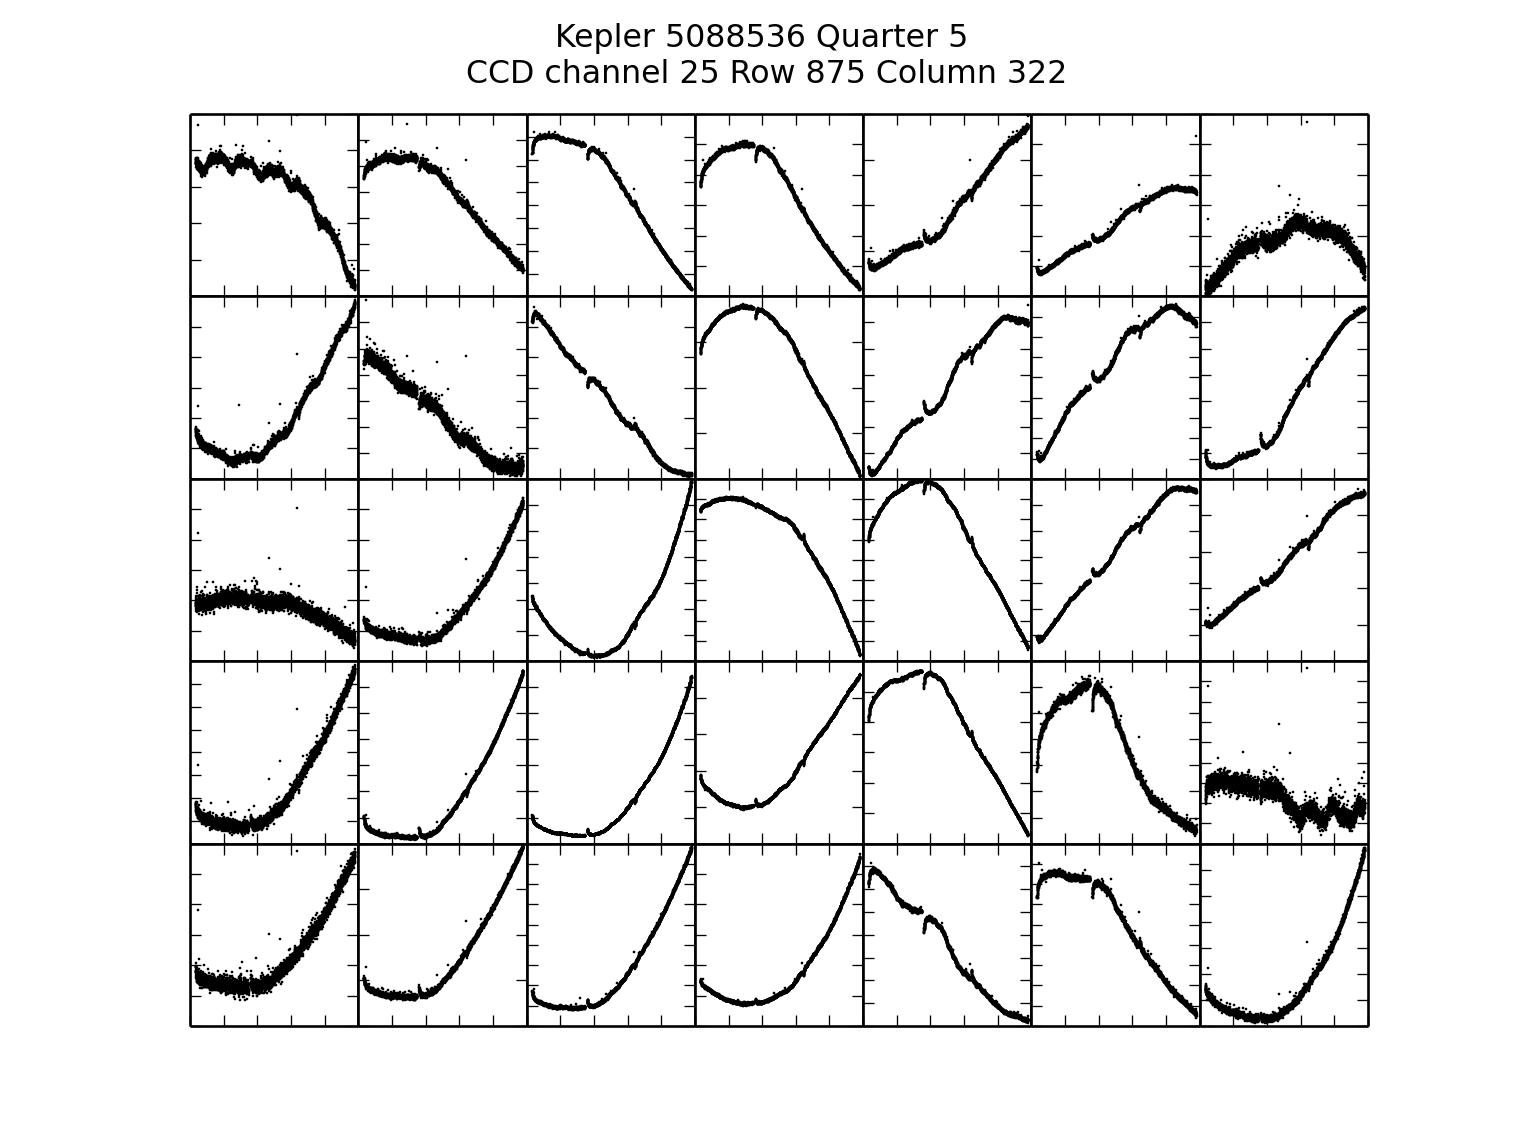
\includegraphics[width=\columnwidth]{5088536-5}
\caption{}
\end{subfigure}%
\hfill
\begin{subfigure}[htb]{0.48\columnwidth}
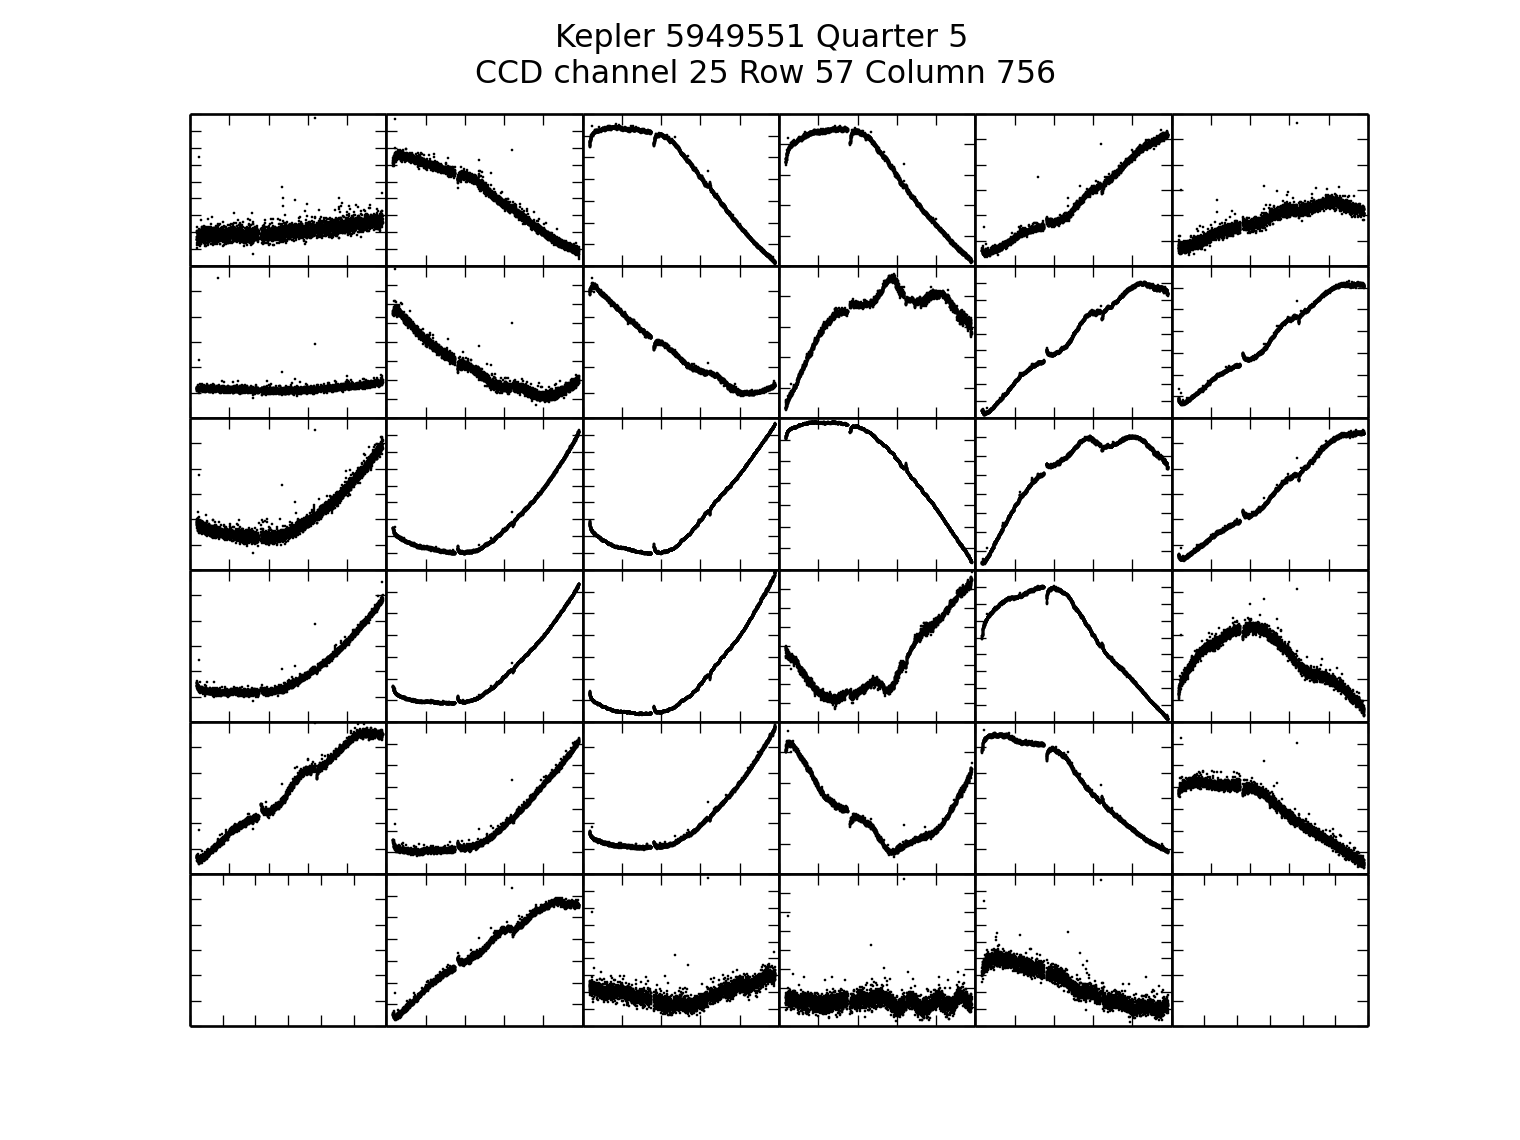
\includegraphics[width=\columnwidth]{5949551-5}
\caption{}
\end{subfigure}
\caption{\label{ccd} Stars on the same CCD share systematic errors. 
The two panels show pixel fluxes (brightnesses) for two stars: (a) KIC 5088536, (b) KIC 5949551; 
here, KIC stands for Kepler Input Catalog. Both stars lie on the same CCD (see Fig.~\ref{fig1}), 
but far enough apart such that there is no stray light from one affecting the other. 
Each panel shows the pixels contributing to the respective star. 
Note that there exist similar trends in these two stars, caused by systematic errors. 
%The idea of our approach is to predict each pixel from a set of pixels from other stars in order to remove those systematics.
}
\end{figure}



The third general idea is that we need to control for over-fitting.
That is, once you have a flexible-enough model you can in principle fit \emph{anything},
  whether it was caused by the spacecraft, intrinsic stellar variability, or a transiting exoplanet.
How do you prevent a very flexible model from taking small noise-induced fluctuations in all the input data
  and carefully combining them linearly into detailed models for every nook and cranny in the target data?
In most projects in astrophysics, over-fitting is controlled for by limiting model freedom.
The model is restricted in the number of parameters
  (as in ``you can't have more parameters than data points'')
  or by limiting the dimensionality
  (as in principal components analysis)
  or by applying strong priors
  (as with smoothness priors, that effectively reduce freedom without explicitly reducing the number of parameters).
In each case, the restriction on model freedom is controlled by some \emph{hyper-parameter}
  (such as the number of inputs, or number of principal components, or the strength of the smoothness prior).
The hyper-parameters can be set or tested with tools like cross-validation,
  the fully marginalized likelihood (Bayes factor or evidence),
  chi-squared statistical criteria,
  or intuition or heuristics.
Here we take a different and more general approach, which is to use a train-and-test framework.

In this framework, the data used to \emph{train} the model%
  ---meaning set the values of the parameters of the model---%
  are disjoint from the \emph{test} data
  ---meaning the data that are being predicted (the target data).
Because we are extremely concerned with detecting Earth-analog exoplanet transits,
  which take about ten hours,
  we adopt an extreme version of the train-and-test framework,
  in which the training data are always separated from the test data by at least ten hours.
That is, when we are using the model to predict a particular pixel in the target data taken at time $t$,
  we use parameters obtained by an optimization that makes use of only data
  that comes either at times prior to $t-\Delta t$ or after $t+\Delta t$,
  where $\Delta t$ is a tunable parameter but which we will set to roughly $12$~h.
This ensures that no information about any exoplanet transit itself
  can be entering into the prediction of the pixels contributing to the stellar photometry.
In general, if there is a scientific goal of preserving intrinsic stellar variability,
  or transit signals,
  on time-scales of $\tau$,
  the parameter optimization ought to be based on training data taken with a time-exclusion zone of half-width $\Delta t > \tau$.

In addition, each training data set within which we set the parameters (by optimization) has a finite total time extent $t_{\max}\approx 30$\,d.
The train-and-test framework, which includes data out to time $t_{\max}$ but excludes data within $\Delta t$ of the test data,
  effectively assumes that the signals worth preserving have time-scales less than $\Delta t$ but don't recur on time-scales
  shorter than $t_{\max}$.
Those assumptions are good for our purposes but not necessarily ideal for all users:
Short-period exoplanets and certain kinds of stellar variability
  could be wiped out by a model with these settings of the training-data regime.

The fourth general idea involved in this kind of data-driven modeling is that the models often aren't \emph{interpretable}, or at least hard to interpret.
This means, in particular, that although the model might do a good job of \emph{predicting} the target pixels,
  using a linear (or more complex) combination of the input pixel data,
  it won't deliver anything that can be unambiguously interpreted as the \emph{flux} of the star in question,
  or any other signal we care about.
The data-driven model \emph{effectively} describes the pointing, point-spread function, and flat-field
  of the telescope and camera,
  plus the variability of every star and every exoplanet transit,
  but it does so without ever \emph{explicitly} creating any of those objects.
We have to make some kind of heuristic or interpretive move to extract from the data-driven model the quanitites of interest.

Finally, the fifth general idea is that there is no objective \emph{ground truth} against which we can tell
  that any particular data-driven model is better or worse than any other.
This problem is a problem for \name, and for the \Kepler\ PDC, and any other data-driven calibration models.
One might think that the ``best'' model is the one that predicts data with lowest variance;
  this would be true if all models adhered to the same train-and-test framework, which they don't.
Besides, a model that can predict not just the spacecraft-induced variability,
  but also variability caused by exoplanet transits of interest,
  will effectively over-fit and distort the most important information in the light-curves.
That is, what is considered best for modeling the data depends on the objectives of the user.
For us, who are interested (in the long term) in finding and characterizing Earth analogs,
  the ``best'' data-driven model is the one that produces the most success in finding and characterizing Earth analogs!
What we will show in what follows is that the \name\ photometry does not distort
  artificial exoplanet transit signals injected into real \Kepler\ pixel-level data.
  and promising properties of the \name\ outputs.
In the end, the value of the \name\ will be demonstrated by the scientific projects it enables.

\Bernhard{Hogg: maybe you want to add sth about the device being 'self-calibratable'?}

\section{\name\ specification and hyper-parameters}
\subsection{\name\ model}
Each individual \Kepler\ target star is, for each quarter (each 90-ish-day period)
  on a particular CCD on the \Kepler\ focal plane.
Associated with each target star is some set of pixels,
  located in a small contiguous patch more-or-less centered on the target star,
  and telemetered down once for every 30-min exposure.
(Here we are ignoring all short-cadence data that is taken in a different mode with shorter exposures.)
That is, each telemetered pixel in each CCD is associated with a particular \Kepler\ target star.

Let's consider a particular pixel $m$ in the focal plane in one particular month
(here we always use data per month rather than quarter,  
since there is discontinuity between every 30-ish-day period).\Bernhard{as an aside: I wonder whether \name reduces these discontinuities at all? (if we were to apply it across the discontinuities)}
In that month, the spacecraft delivers $N\sim 1300$ measurements $I_{m,n}$
  of the intensity falling in that pixel at the $N$ times $t_n$ at which exposures were taken during the month.
(For intensity measurements $I_{m,n}$ here we are using pixels from the Target Pixel Files.\Bernhard{include reference})
We want to build a prediction for the intensity $I_{m,n}$ in pixel $m$ at each time $t_n$
  using the intensities $I_{m',n}$ of other pixels $m'$.
The question is:  What other pixels to choose?
There are many possible qualitatively and quantitatively different choices here.
Assuming that they are affected by similar systematic errors as the target star pixels, we choose all the pixels $m'$ associated with the $Q$ stars on the same CCD in the same quarter
  that are closest in magnitude
  (\Kepler\ magnitude as reported in the \Kepler\ Input Catalog)
  to the target star associated with pixel $m$.
This set of pixels%
  ---from the $Q$ stars on the same CCD---%
  is the \emph{pixel set} $\set{M}_m$ associated with pixel $m$.
   To rule out any direct optical cross-talk by starry 
light, we require that the predictor pixels are from stars
sufficiently far away from the target star (at least 20 pixels distance on the CCD).
Note that because the set $\set{M}_m$ is of pixels associated with \emph{different} stars
  than the star associated with pixel $m$, and are far from it on CCD, 
  the pixel $m$ will not be in the set $\set{M}_m$,
  and nor will any of pixel $m$'s close neighbors.
That is, there will be no (or almost no) overlap in stellar illumination of pixel $m$
  and the pixels $m'\in\set{M}_m$.

When we are predicting the measurement $I_{m,n}$ from pixel $m$ at a particular time $t_n$,
  we are going to use a train-and-test framework in which not only do we not use
  data at time $t_n$ in optimizing the parameters of the regression or fit,
  but we don't even use any times $t$ such that $|t-t_n| < \Delta t$,
  where $\Delta t\sim 10$\,h as shown in Fig.~\ref{train-and-test}.
That is, we train (optimize fit parameters) using the \emph{time set} $\set{N}_n$ of time
  indices $n'$ such that for all $n'\in\set{N}_n$,
  $t_{n'}$ is in the same quarter as $t_n$,
  and $|t_{n'} - t_n|>\Delta t$.
The time set of indices $\set{N}_n$ therefore does not overlap the time point $t_n$,
  nor any of its neighbors in a time window of half-width $\Delta_t$. 
  
\begin{figure}[htb]
\centering
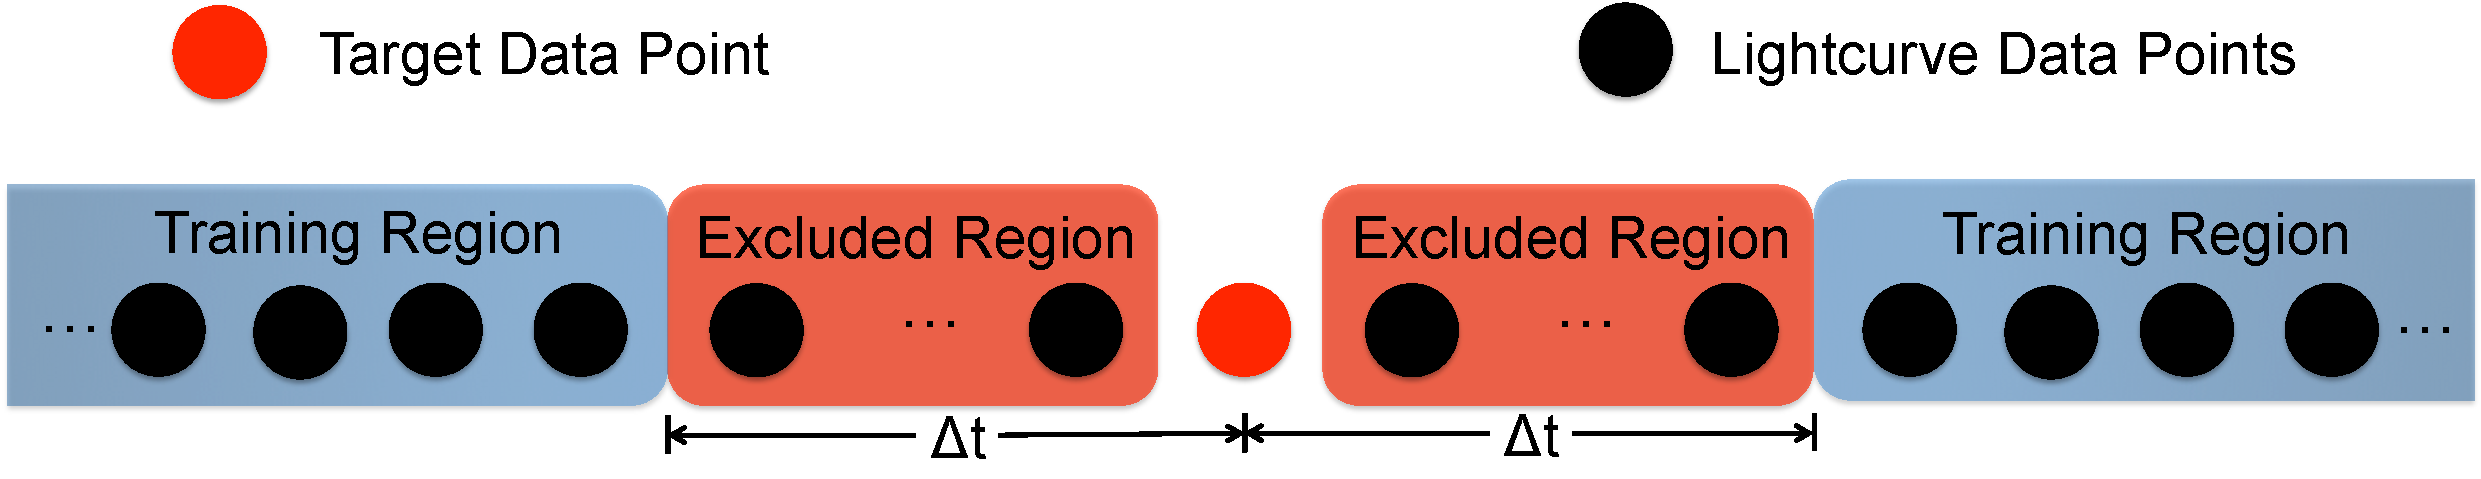
\includegraphics[width=0.8\columnwidth]{train_and_test}
\caption{\label{train-and-test} Train-and-test framework. Data near the target point $t_{n}$ within $\Delta t$ is excluded in the training set}
\end{figure}

In addition to pixel set $m'\in\set{M}_m$ from other stars,  
  we also include past and future of the target star --- autoregressive (AR) component as input 
  to remove more of the stellar variability and thus increase the sensitivity for transits. 
To do this, we select an exclusion window of half-width $\Delta t$ including R data points, 
  where $\Delta t\sim 10$\, h (as big as the window in the train-and-test framework) 
  around the point of time $t_{n}$ being corrected, 
  to ensure that we do not remove the transit itself and then use $S$ closest future and past time points. 
That is, for every pixel $m$ in the target star , we construct $S$ virtual time series, 
  in which every component $v$ is defined to be     
\begin{eqnarray}
I_{v,n} = I_{m,n-R-k}\ or\ I_{v,n} = I_{m,n+R+k},
\quad,
\end{eqnarray}
\Bernhard{I find the notation $I_{mn-R-k}$ confusing --- better write $I_{m,n-R-k}$, and then for consistency also $I_{v,n}$ etc.}
where $k = 0, 1,\dots, S,$ so if there are totally $M$ pixels in the target stars, 
  we will finally add $2\cdot M\cdot S$\Bernhard{not quite: if I am right, then there are overall $(2R-1)$ in the exclusion zone, and $2S+2$ are used, for each pixel} autoregressive components into the predictors, 
  which constructs the autoregressive set $\set{V}_m$

As mentioned above, in the context of this project,
  a model is something that can predict data given settings of some parameters,
  and an objective function that can be used to find best values for those parameters.
It is often preferable to work in a probabilistic mode in which the objective function can be justified
  in terms of a likelihood (probability for the data given the model)
  or a posterior probability density function (likelihood times a prior pdf).
The \name\ treats each \Kepler\ data point $I_{m,n}$ as being
  predictable from a linear combination of data points $I_{m',n}$,
  where $m'$ is from the set of non-overlapping pixels $m'\in\set{M}_m$.
\begin{eqnarray}
I_{m,n}         &=& I^{\ast}_{m,n} + e_{m,n}
\\
I^{\ast}_{m,n}  &=& \sum_{m'\in\set{M}_m} a_{mnm'}\,I_{m',n} + \sum_{v\in\set{V}_m} b_{mnv}\,I_{v,n}
\quad,
\end{eqnarray}
where $I^{\ast}_{m,n}$ is the prediction (by the model) for data point $I_{m,n}$,
  $e_{m,n}$ is a noise contribution or residual away from the prediction,
  and the $a_{mnm'}$ and $b_{mnk}$ are the parameters (linear coefficients of the prediction).
The parameters $a_{mnm'}$ and $b_{mnk}$ have indices $m$ because
  they are different for every pixel $m$,
  and they will even be different for every time step $n$;
  that is, there will be a separate best-fit value for the parameters for every $I_{m,n}$.
If we presume that the residuals away from the prediction are normally distributed with zero mean
  and known variance,
  likelihood optimization reduces to $\chi^2$ \Bernhard{maybe better $\chi^2$?} minimization.
We add to the standard chi-squared definition a regularization term
  (equivalent to multiplying the likelihood by a Gaussian prior pdf)
  that penalizes large absolute values for the the coefficients $a_{mnm'}$:
\begin{eqnarray}
\chi^2_{m,n}    &=& \sum_{n'\in\set{N}_n} \frac{[I_{m,n'} - I^{\ast}_{m,n',n}]^2}{\sigma^2_{m,n'}}
                 + \lambda_{a}\sum_{m'\in\set{M}_m}a_{mnm'}^2 + \lambda_{b}\sum_{v\in\set{V}_m}b_{mnv}^2
\\
I^{\ast}_{m,n',n} &=& \sum_{m'\in\set{M}_m} a_{mnm'}\,I_{m',n'} + \sum_{v\in\set{V}_m} b_{mnv}\,I_{v,n'}
\quad,
\end{eqnarray}
\Bernhard{(1) why does $I$ have three indices now, and what does that mean? In Eq. (3) there are only two indices. (2) do we need the sigmas at all, or could we absord this into the lambdas?}
\Dun{In CPM,  for every time points,  the $\chi^2$ minimization is independent, the third index of $I^{\ast}$ indicates which time point is being 
optimized,  maybe I can find a better notation}
where the $\sigma^2_{m,n'}$ are the (presumed known)\Bernhard{known, or estimated from data? If not estimated, how do we know them?} individual-pixel noise variances,
  and $\lambda_{a}$, $\lambda_{b}$ set the strength of the regularization (or width of the prior pdf) for parameters $a_{mnm'}, b_{mnv}$. In general, $\lambda_a$ and $\lambda_b$ could depend on $m,n$, however, we do not make use of this freedom.

The train-and-test idea comes into the objective function $\chi^2_{m,n}$:
When we are computing the objective function $\chi^2_{m,n}$,
  we are using only time points $n'\in\set{N}_n$ that don't overlap the target (or test) time point $n$.
We train the model---that is, set the parameters $a_{mnm'}$ and $b_{mnv}$---%
  by choosing the full set of parameters that jointly minimize the objective function $\chi^2_{m,n}$.
Fortunately, given the form of the model,
  this minimization is just a linear solve (linear operation on the data).
Importantly however, and perhaps surprisingly, the objective function $\chi^2_{m,n}$ is \emph{different}
  for every target data point (pixel value to be predicted) $I_{m,n}$;
  we have to do an \emph{independent optimization} (or really linear solve)
  of the parameters for every pixel value we want to predict.
That is, every pixel datum $I_{m,n}$ we predict will have
  \emph{different} settings of the parameters $a_{mnm'}$ and $b_{mnk}$.
Since there are of order $10^{6}$ total pixel values in the \Kepler\ Target Pixel Files for \emph{each \Kepler\ target},
  and of order $10^7$ data sources used as basis functions in the linear fitting,
  this represents one fuck of a lot of linear solves,
  and a lot of parameters to obtain and record.

Once we have obtained the parameters $a_{mnm'}$ and $b_{mnv}$ corresponding to a particular data point $I_{m,n}$,
  we can make a \emph{prediction} $I^{\ast}_{m,n}$ for the intensity at that pixel.
By construction of our objective function, this is truly a prediction,
  in the sense that the optimization (or solve) that produced the parameters
  (and thus the prediction)
  did not make use of $I_{m,n}$ itself,
  or even any of the pixel values that are nearby in angle or time
  (as described above).
  With all the predicted pixel values $I^{\ast}_{m,n}$ of the target star,  
  our new stellar flux estimates,
  what we will call the ``\name\ prediction'',
  is constructed from the \name\ pixels
  in precisely the same way as the official \Kepler\ SAP photometry
  is constructed from the Target Pixel Files.
That is, we perform a weighted sum of \name\ predicted pixels $I^{\ast}_{m,n}$ with weights $w_m$,
  all of which are either zero or unity,
  and we adopt precisely the same weight assignments as are adopted in the SAP photometry;
  in equations, the flux estimate $S_n$ at time $t_n$ of the target star is given by
\begin{eqnarray}
S_n = \sum_m w_m\,I^{\ast}_{m,n}
\quad ,
\end{eqnarray}
where the sum is over the $M$ pixels that are associated with the target star and the weight $w_m$ is unity for pixels in the optimal
aperture while zero outside the optimal aperture.
 \Bernhard{if the sum is only over the pixels of the target star, then all $w_m$ are equal to 1 and they can be dropped}.
As we have noted above and below, these photometric estimators are not optimal for any purpose,
  but improving them is beyond the scope of this project.

It is worth to mention that the \name\ prediction $S_{n}$ is constructed from pixels without any information about transits in the target star.\Bernhard{changed this --- I didn't understand it} Therefore, it can be regarded as a light curve without transit signal. 
Based on this idea, 
  we can construct the ``\name\ flux'' (where the inverted commas indicate that it is not a flux in the sense that stellar variability is not preserved) to be the relative residual between \name\ prediction and SAP Flux $F_{n}$
\begin{eqnarray}
\delta_{n}&\equiv&\frac{F_{n} - S_{n}}{S_{n}}
\quad .
\end{eqnarray}
The \name\ flux is 
In some sense, it is this relative residual that contains the exoplanet transit signals we seek. 
That is, a transit creates a negative residual away from the prediction, 
  and the amount of relative residual is just the fraction of the light eclipsed by the planet (the transit depth). 

\subsection{Hyper-parameters}
In the description of \name, 
  we introduce 4 hyper-parameters---number of predictor stars Q (or number of predictor pixels P), 
  number of autoregressive components S, and the two regularization strength $\lambda_{a}$ and $\lambda_{b}$.
To set these 4 hyper-parameters, 
  in principle we need to run cross-validation on every single star to optimize the performance of \name.
But optimizing in this 4-dimensional space is expensive, 
  especially in \name\ we need to solve thousands of linear systems with thousands of parameters. 
Therefore, in this paper, 
  we just set a general set of ``default'' hyper-parameters ($P=4000$, $Q=3$, $\lambda_a=1e5$, $\lambda_a=1e5$), 
  which works well in most of the stars without highly variability. 
To show how this general set of hyper-parameters performs, 
  here we present a typical comparison between optimized and default hyper-parameters 
  in Fig~\ref{hyperparameter}.\Bernhard{maybe explain somewhere how SNR is calculated}  
We can see that, in Fig~\ref{hyperparameter}, 
  there is less variation in the \name\ flux from optimized hyper-parameters (green points in second panel) 
  than from the default one (red points in the bottom panel). 
In addition, the optimized flux has higher signal to noise ratio of the known transit than the default. 
However, the performance of default hyper-parameters is acceptable 
  and we will use this set of hyper-parameters throughout rest of the paper 
  to show the general performance of \name.

\begin{figure}[htb]
\centering
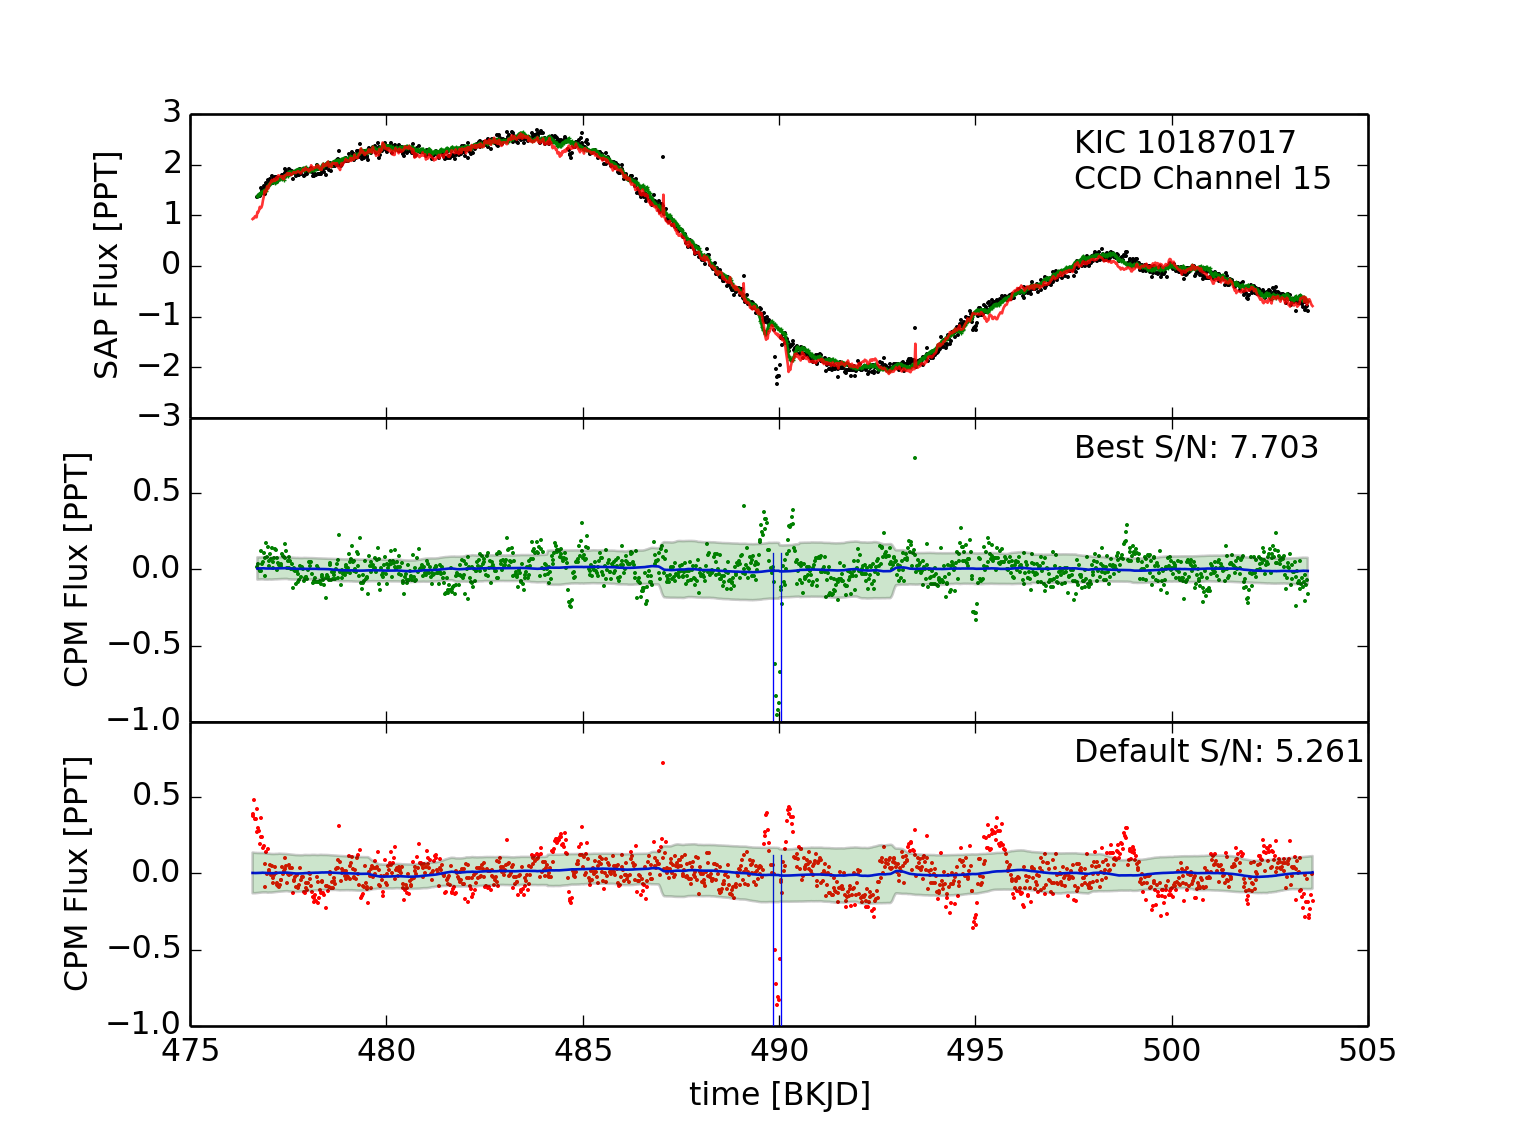
\includegraphics[width=\columnwidth]{compare_10187017}
\caption{\label{hyperparameter} Comparison between default and optimized hyper-parameters. 
In the top panel, SAP flux is plotted in black, \name\ prediction of default hyper parameters is in red line, 
\name\ prediction of optimized hyper-parameters is in green line. 
The middle panel shows the CPM flux of the optimized hyper-parameters, 
while CPM flux of the default hyper-parameters is in the bottom panel, 
the two vertical blue lines indicate the location of the transit signal, and signal to noise ratio is calculated in both situation. 
The optimized hyper-parameter performs better than the default one, but the results from both situation are close.}
\end{figure}

\clearpage

\subsection{Transit signal in \name}
One important feature of \name\ is that we use the train-and-test framework to preserve 
the transit signal. To show how well train-and-test framework performs, we make the
following experiments on \Kepler\ data as shown in Fig~\ref{distortion}
In the light curve of single pixel (1, 2) of KIC 9822284, a 10-hrs fake signal 
with amplitude 1.0005 is inserted. To insert the signal, we simply multiply the light curve 
by the factor of 1.0005, which makes the little bump in the middle of the SAP light curve 
(black points in the first panel). With the distorted light curve, we both applied the 
\name\ and ordinary fitting to the data. In the result, we can see that both \name and 
ordinary fit the light curve quite well outside the range of inserted signal. However, 
when examine how these two models preserve the signal that we care, the ordinary
fitting fit out about 30 percent of the signal, while \name\ almost preserve the whole 
original amplitude. Therefore,  by this simple experiment, we are able to show that 
the train-and-test framework used here is capable to keep the transit signal with 
a particular time scale. And we want to emphasise that it is crucial for searching for
exoplanets, especially the small ones such as earth-like planets, which only have  
about tens of parts per million signal in the light curve.

\begin{figure}[htb]
\centering
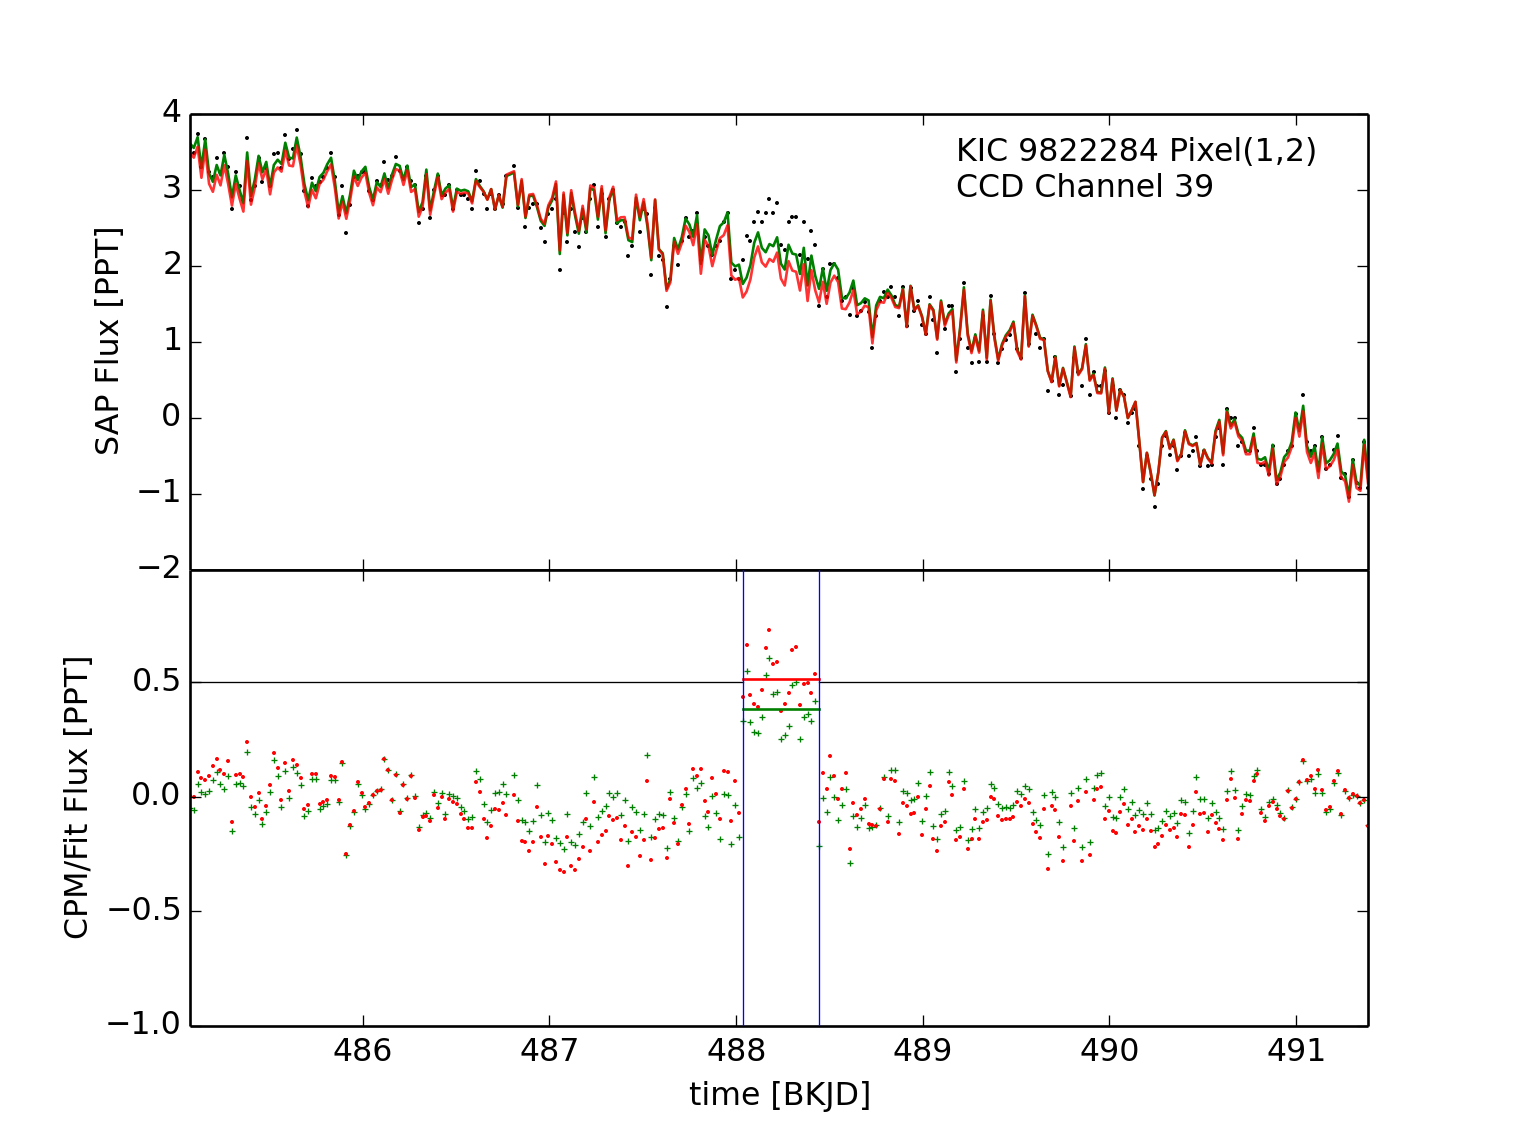
\includegraphics[width=\columnwidth]{distortion_9822284_normal}
\caption{\label{distortion} \name\ preserves transit signals. 
Fake signal with amplitude 1.0005 is inserted into the single pixel (1, 2) of star KIC 9822284. 
In the top panel, the black points shows the SAP flux of the pixel with the injected signal, 
the green line is the fitting of the SAP flux, and the red line is the \name\ prediction. 
In the bottom panel, red and green points represent the \name\ flux and fit flux, 
while the signal value is indicated by the horizontal line. 
CPM largely preserves the signal while the fitting flux overfit the signal.}
\end{figure}

\clearpage

\section{Examples and results}

To give a view on how our method performs, \name\ is applied on several stars with 
known transit signals but different variability and magnitudes as shown in Fig.~\ref{fluxes}. 
From the plots, we can see that \name\ works quite well on these stars, producing the \name\ fluxes 
with low variation and preserving the transit signals.
In addition, \name\ and PDC are compared based on 6 quiet stars 
(non-variable stars, first two rows of Fig.~\ref{fluxes}). 
The results illustrate that for these quiet stars our approach removes 
a major part of the variability present in the PDC light curves, while preserving the transit signals. 
To provide a quantitative comparison, we ran \name\ on 1000 stars from the whole Kepler input catalog 
(500 chosen randomly from the whole list, and 500 random G-type sun-like stars), 
and estimate the Combined Differential Photometric Precision (CDPP) (\todo{citation}) for \name\ and PDC. 
CDPP is an estimate of the relative precision in a time window, 
indicating the noise level seen by a transit signal with a given duration. 
The duration is typically chosen to be 3, 6, or 12 hours. 
We use the 12-hours CDPP metric, since the transit duration of an earth-like planet is roughly 10 hours. 
Before CDPP is estimated, the 100 most variable stars in the list are removed, 
since PDC is not designed to remove stellar variability, and we want to compare \name\ and PDC on the same footing.
Fig.~\ref{cdpp} presents our CDPP comparison of \name\ and PDC, showing that our method (\name) outperforms PDC. 

\begin{figure}[htb]
\centering
\begin{subfigure}[htb]{0.33\textwidth}
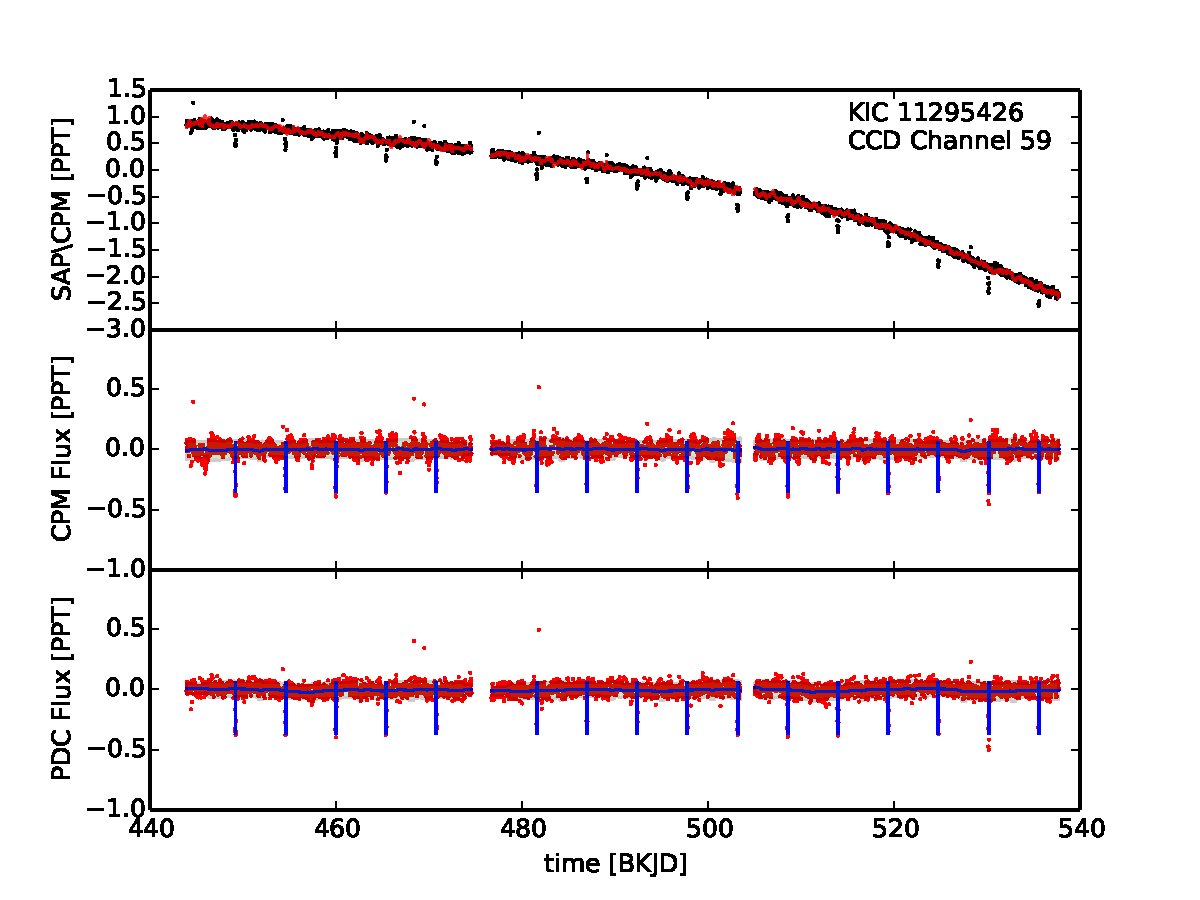
\includegraphics[width=\textwidth]{kic_11295426_pdc}
\end{subfigure}%
\hfill
\begin{subfigure}[htb]{0.33\textwidth}
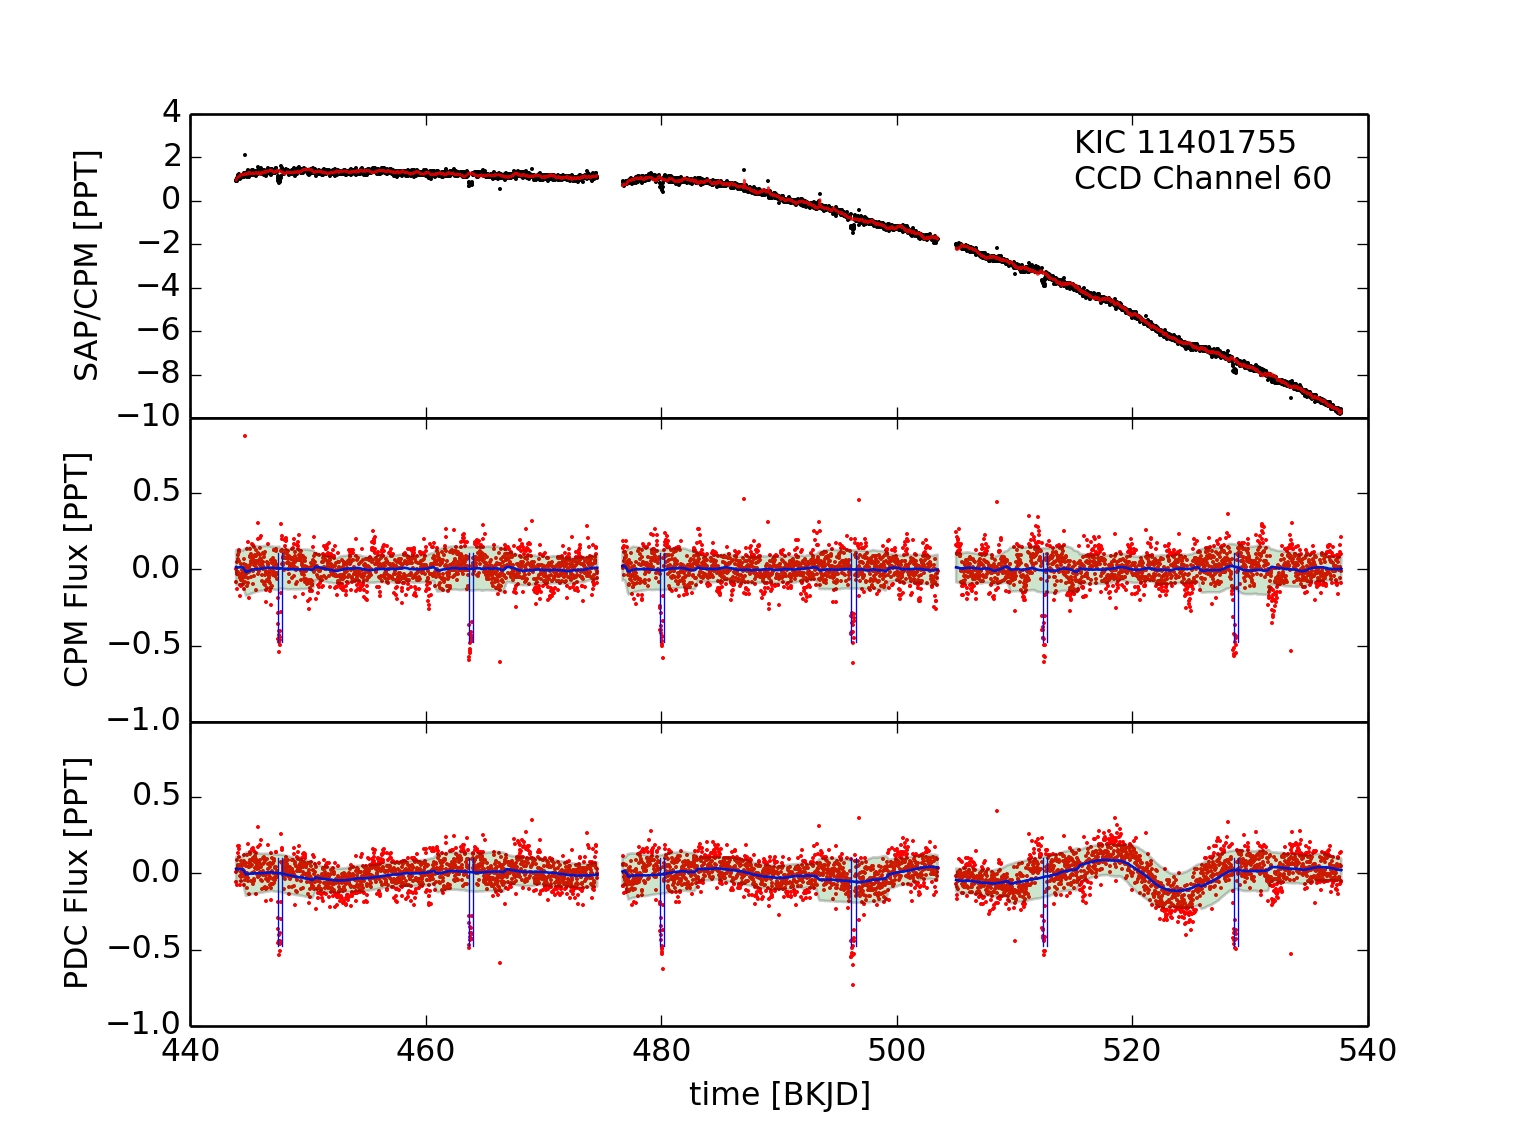
\includegraphics[width=\textwidth]{kic_11401755_pdc}
\end{subfigure}%
\hfill
\begin{subfigure}[htb]{0.33\textwidth}
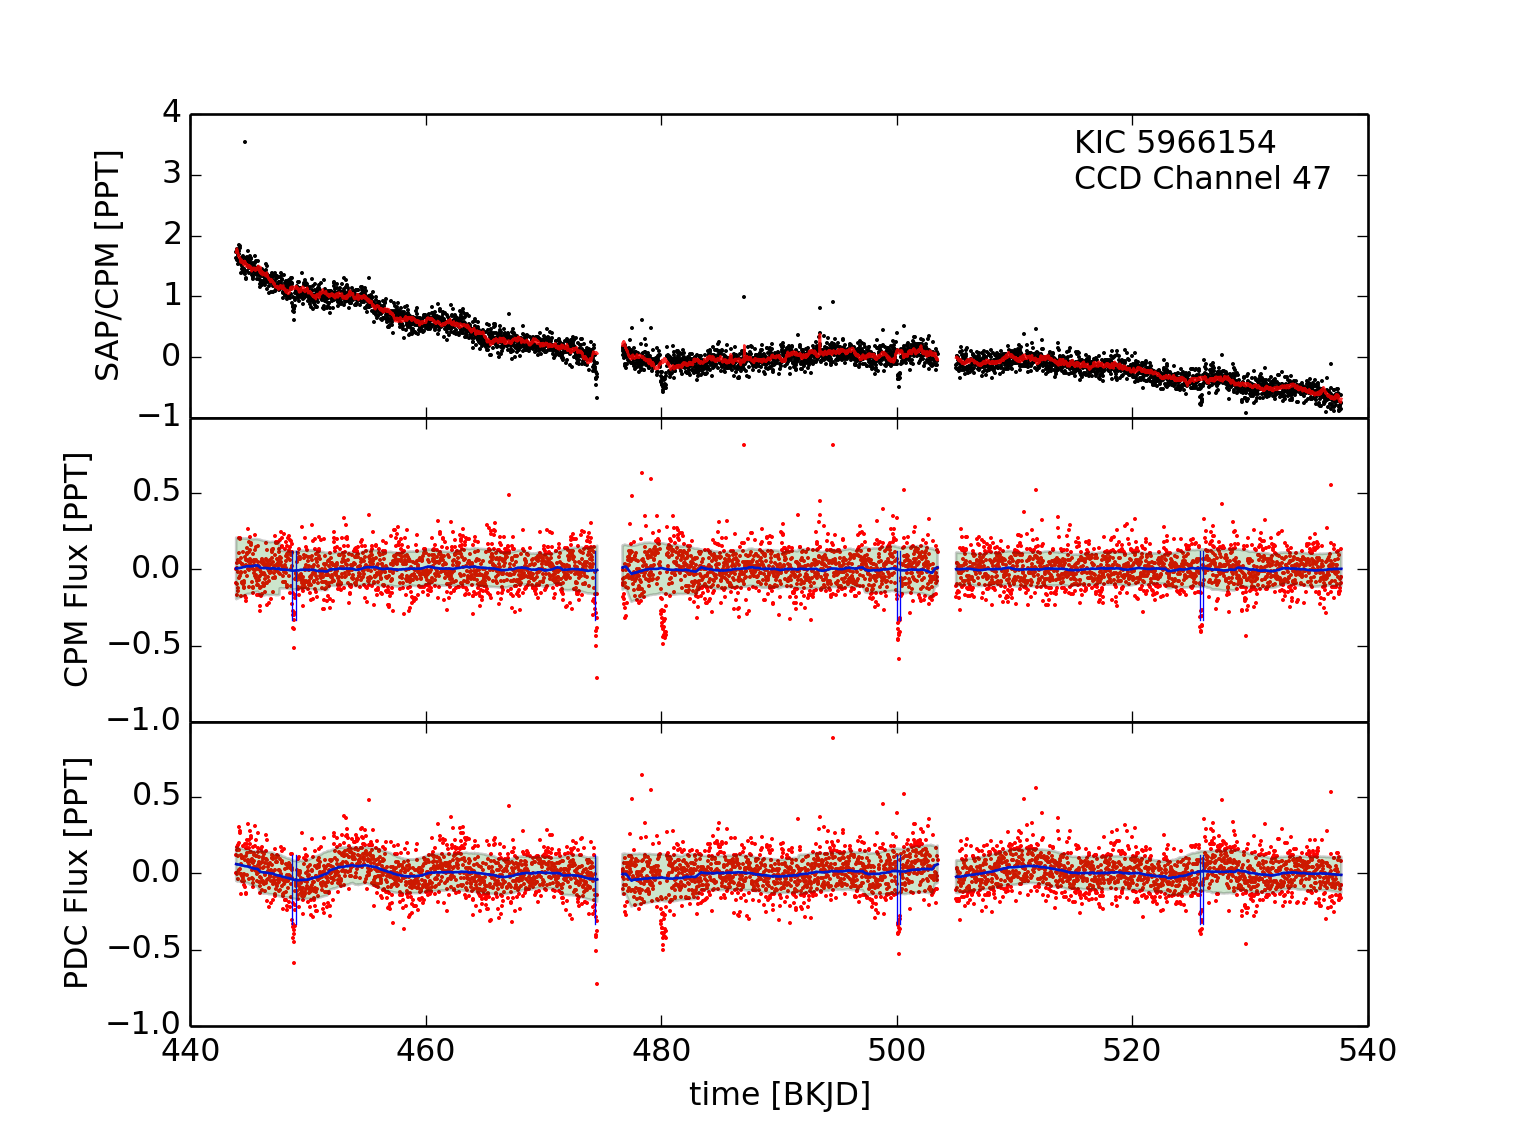
\includegraphics[width=\textwidth]{kic_5966154_pdc}
\end{subfigure}

\begin{subfigure}[htb]{0.33\textwidth}
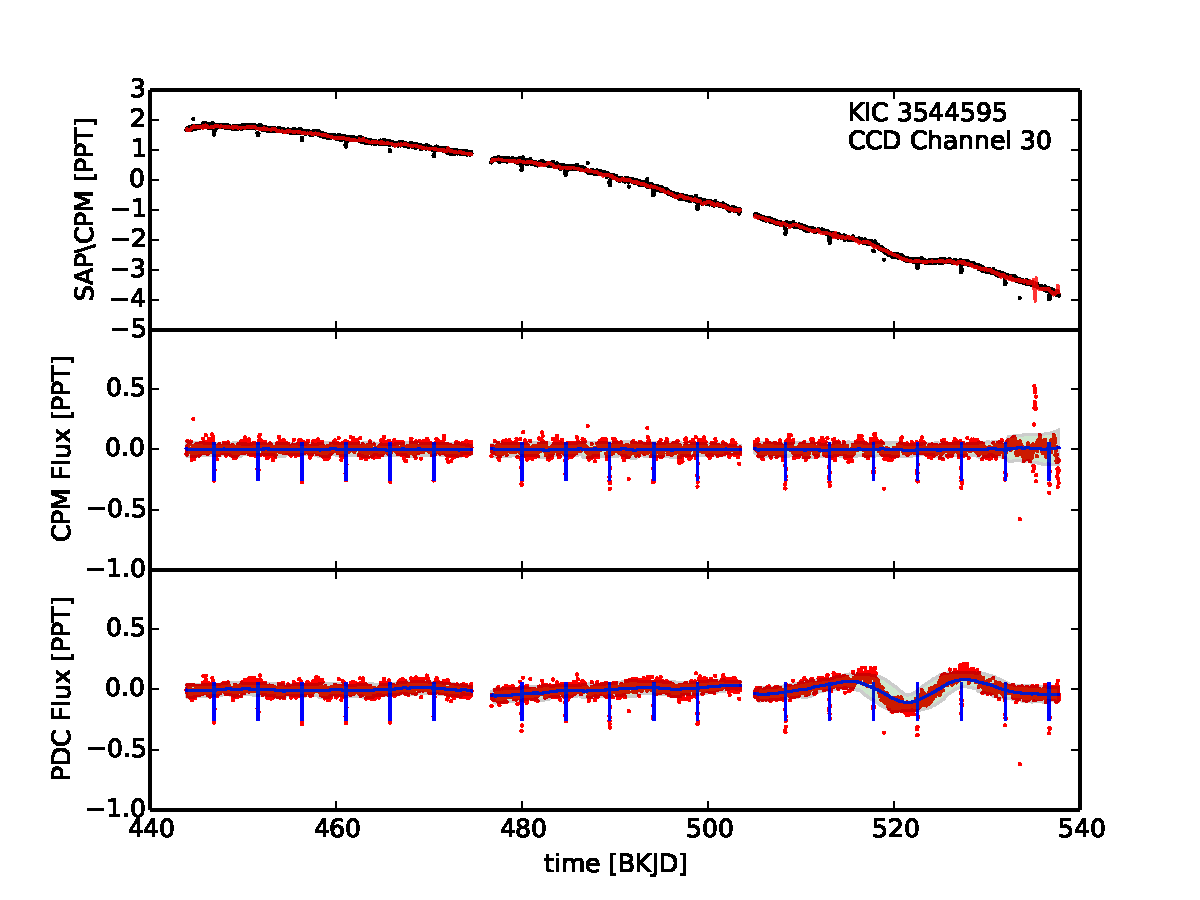
\includegraphics[width=\textwidth]{kic_3544595_pdc}
\end{subfigure}%
\hfill
\begin{subfigure}[htb]{0.33\textwidth}
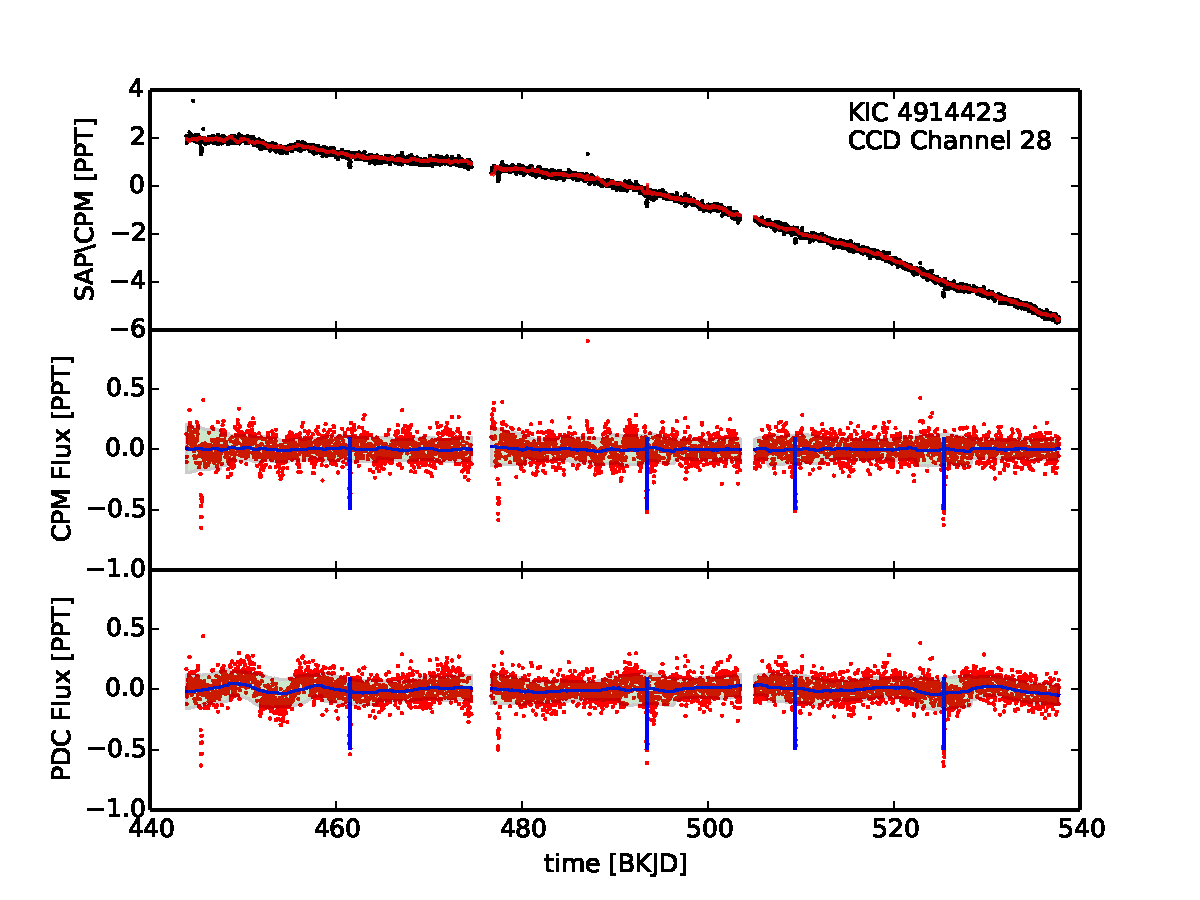
\includegraphics[width=\textwidth]{kic_4914423_pdc}
\end{subfigure}%
\hfill
\begin{subfigure}[htb]{0.33\textwidth}
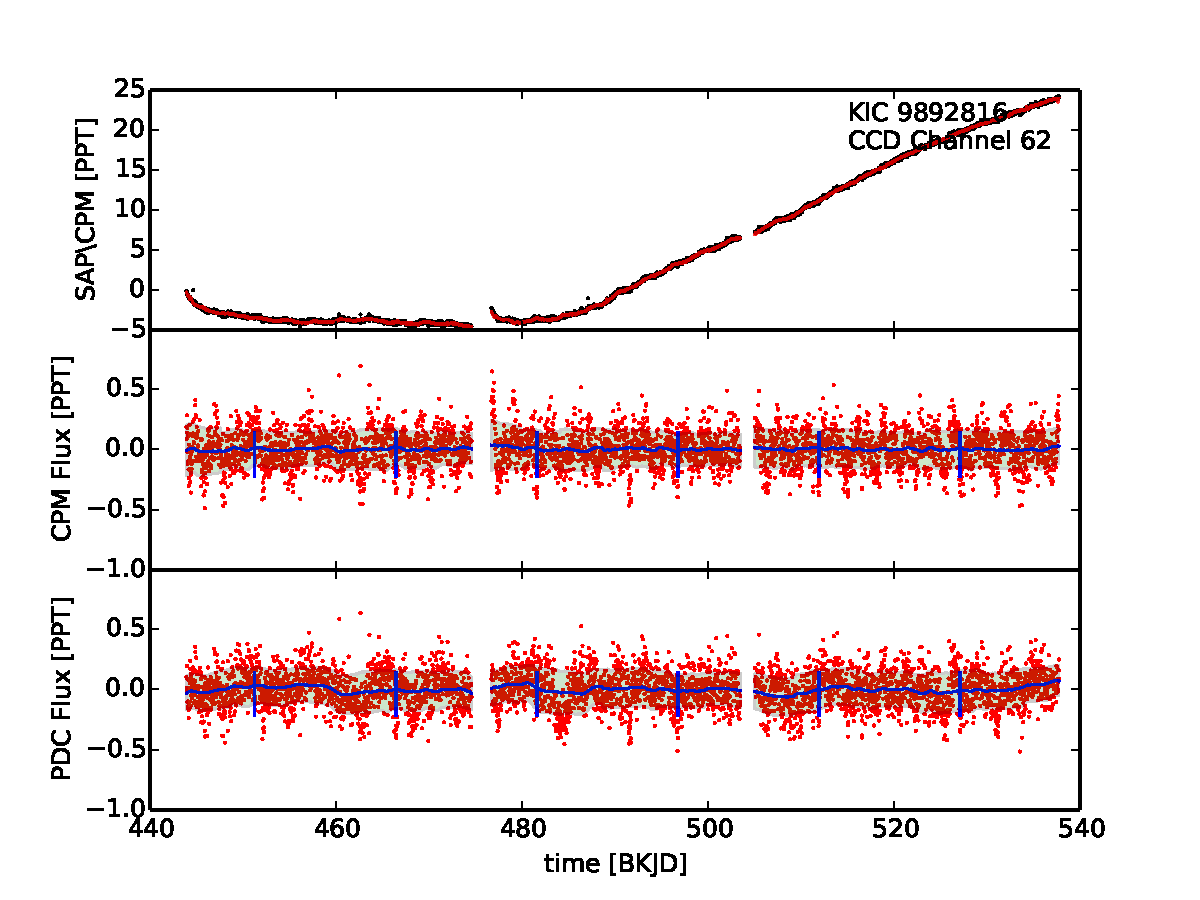
\includegraphics[width=\textwidth]{kic_9892816_pdc}
\end{subfigure}

\begin{subfigure}[htb]{0.33\textwidth}
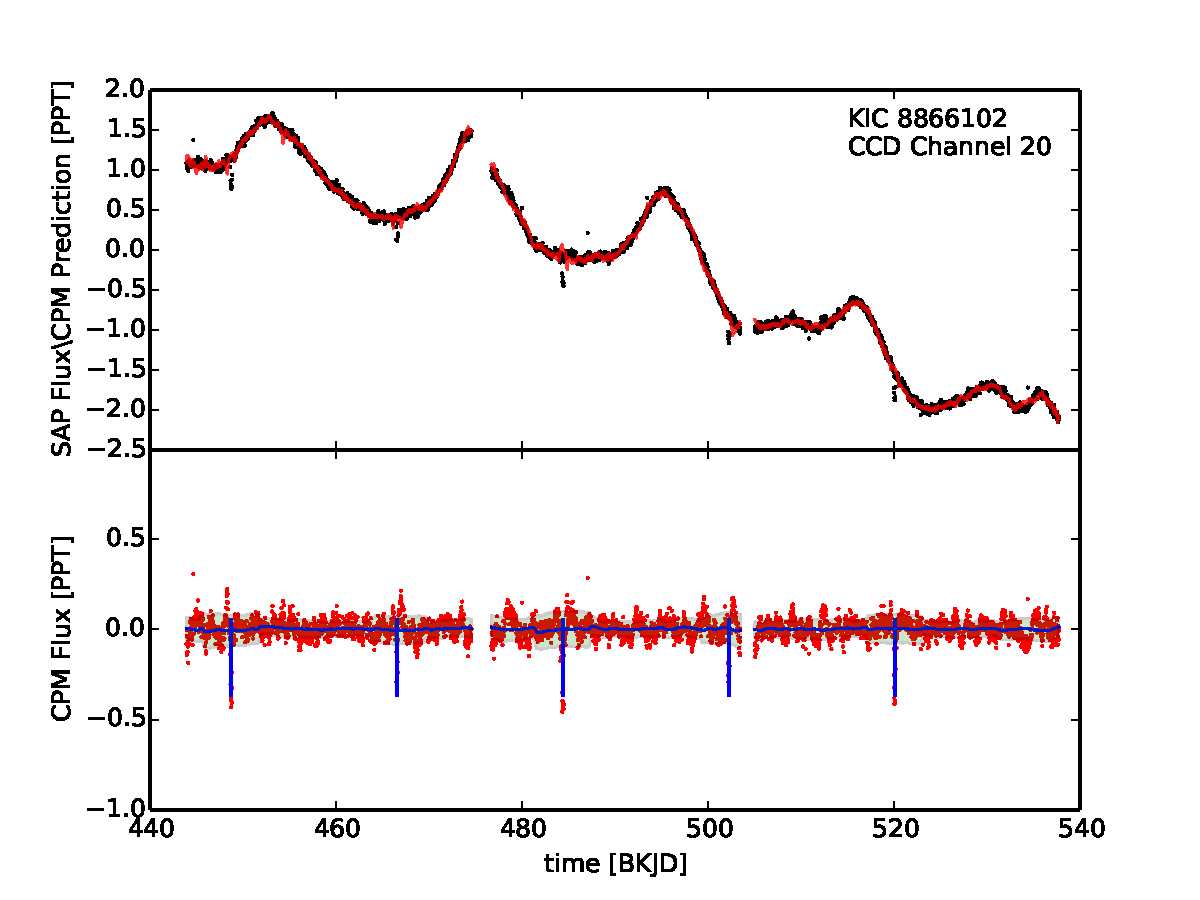
\includegraphics[width=\textwidth]{kic_8866102}
\end{subfigure}%
\hfill
\begin{subfigure}[htb]{0.33\textwidth}
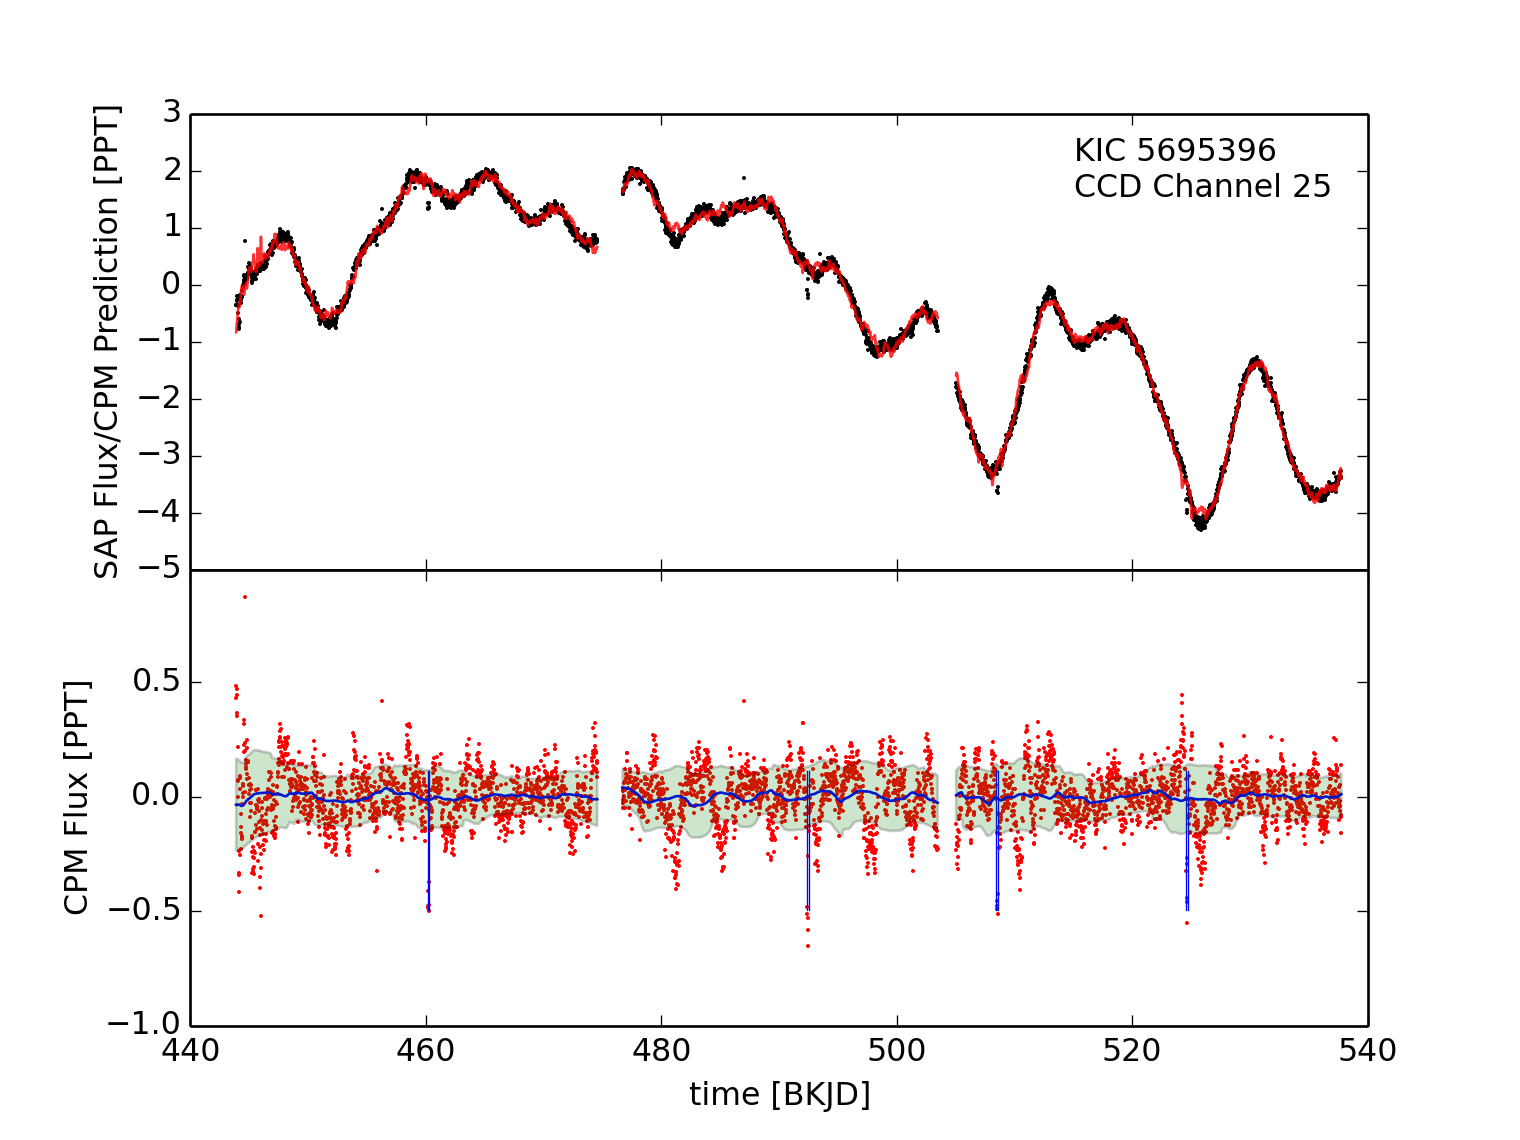
\includegraphics[width=\textwidth]{kic_5695396}
\end{subfigure}%
\hfill
\begin{subfigure}[htb]{0.33\textwidth}
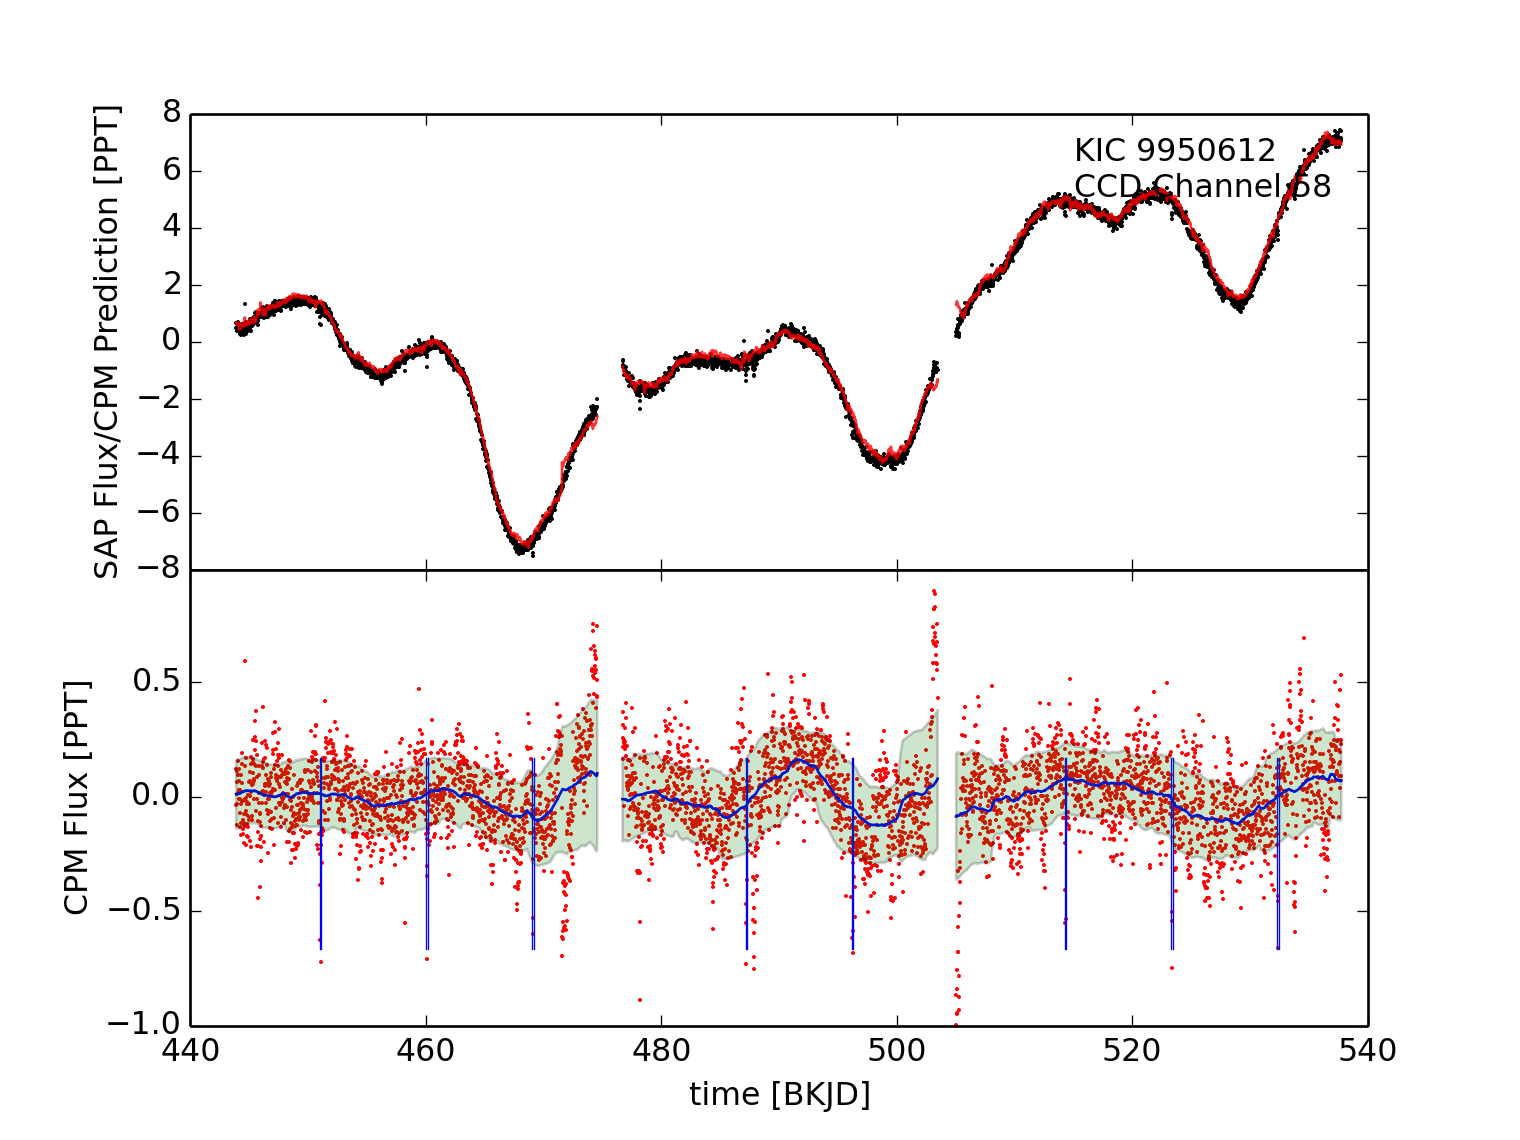
\includegraphics[width=\textwidth]{kic_9950612}
\end{subfigure}
\begin{subfigure}[htb]{0.33\textwidth}
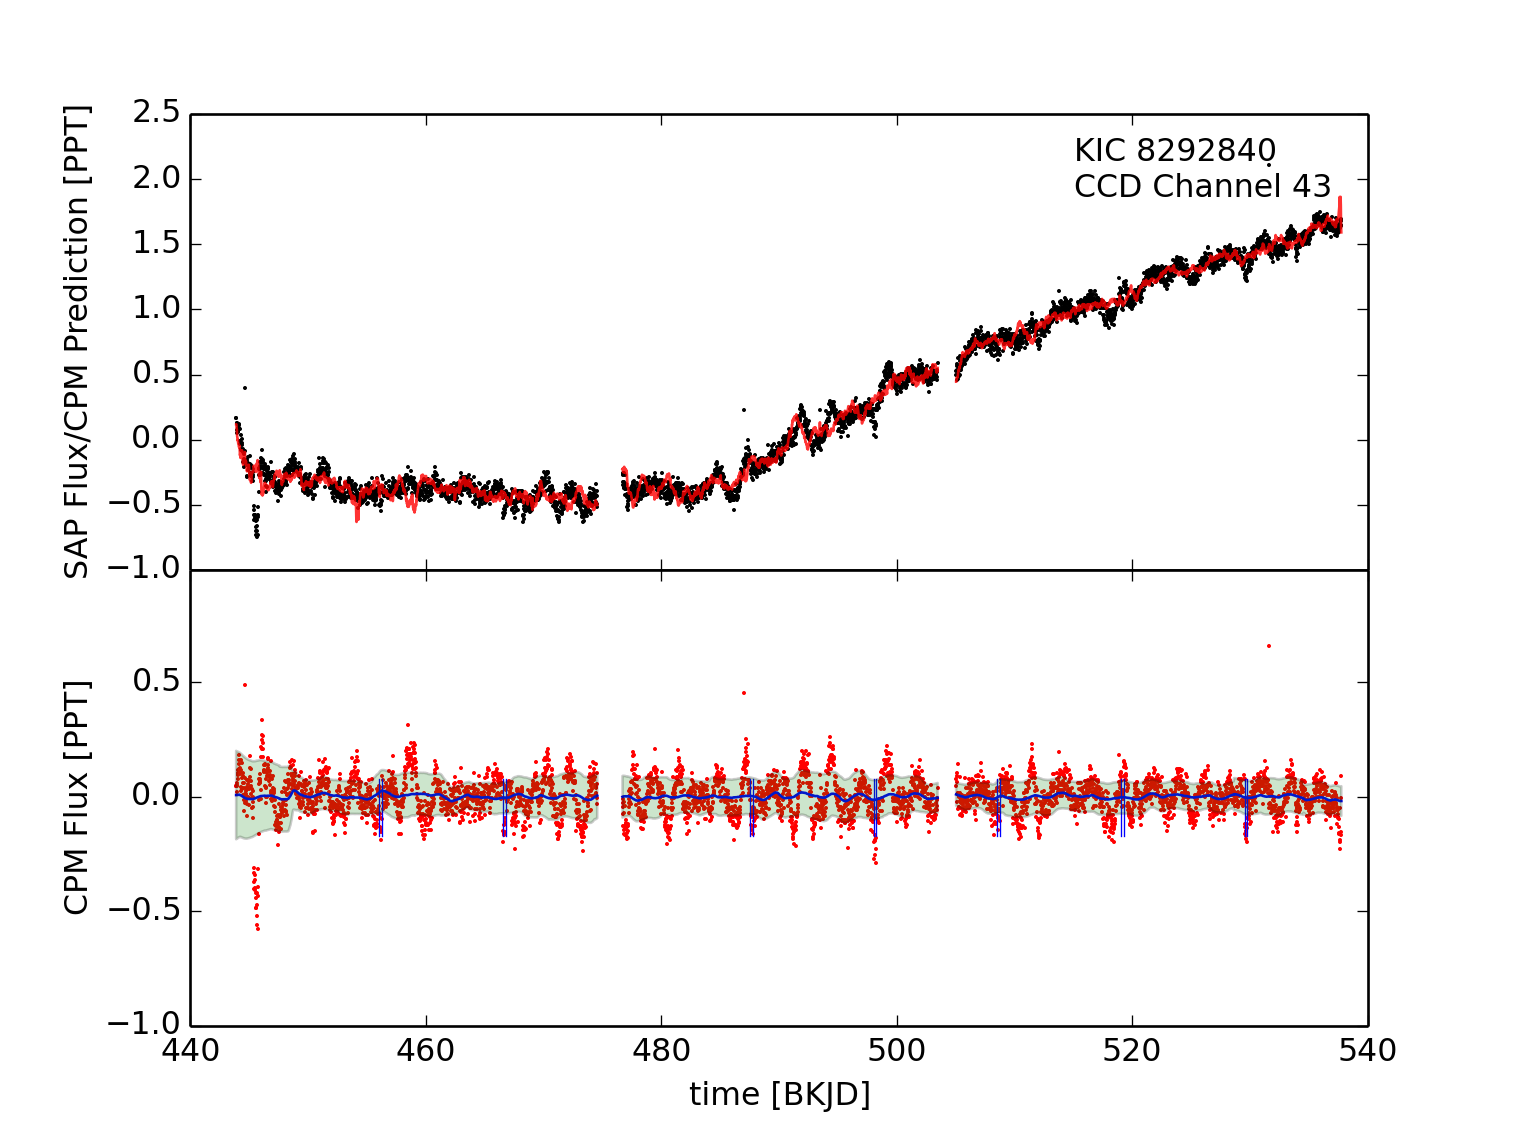
\includegraphics[width=\textwidth]{kic_8292840}
\end{subfigure}%
\hfill
\begin{subfigure}[htb]{0.33\textwidth}
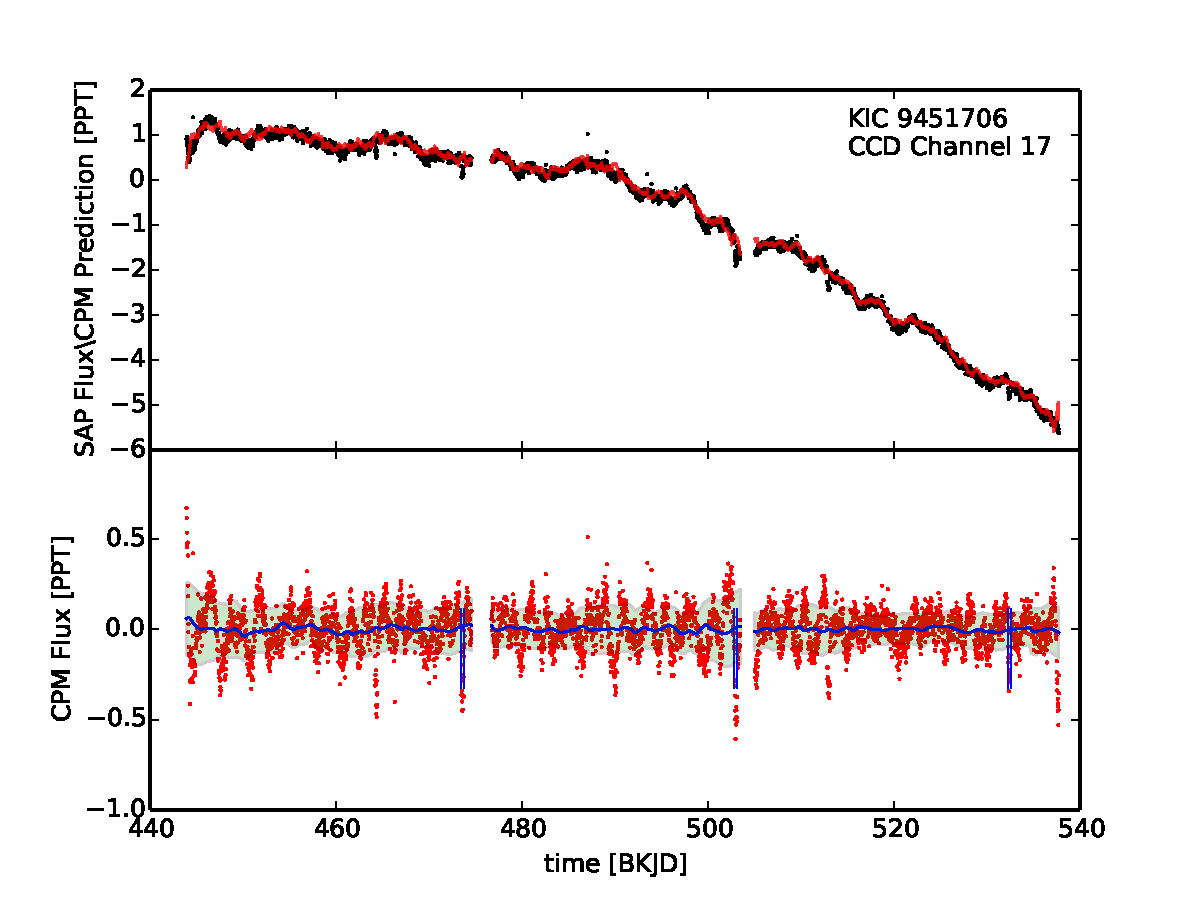
\includegraphics[width=\textwidth]{kic_9451706}
\end{subfigure}%
\hfill
\begin{subfigure}[htb]{0.33\textwidth}
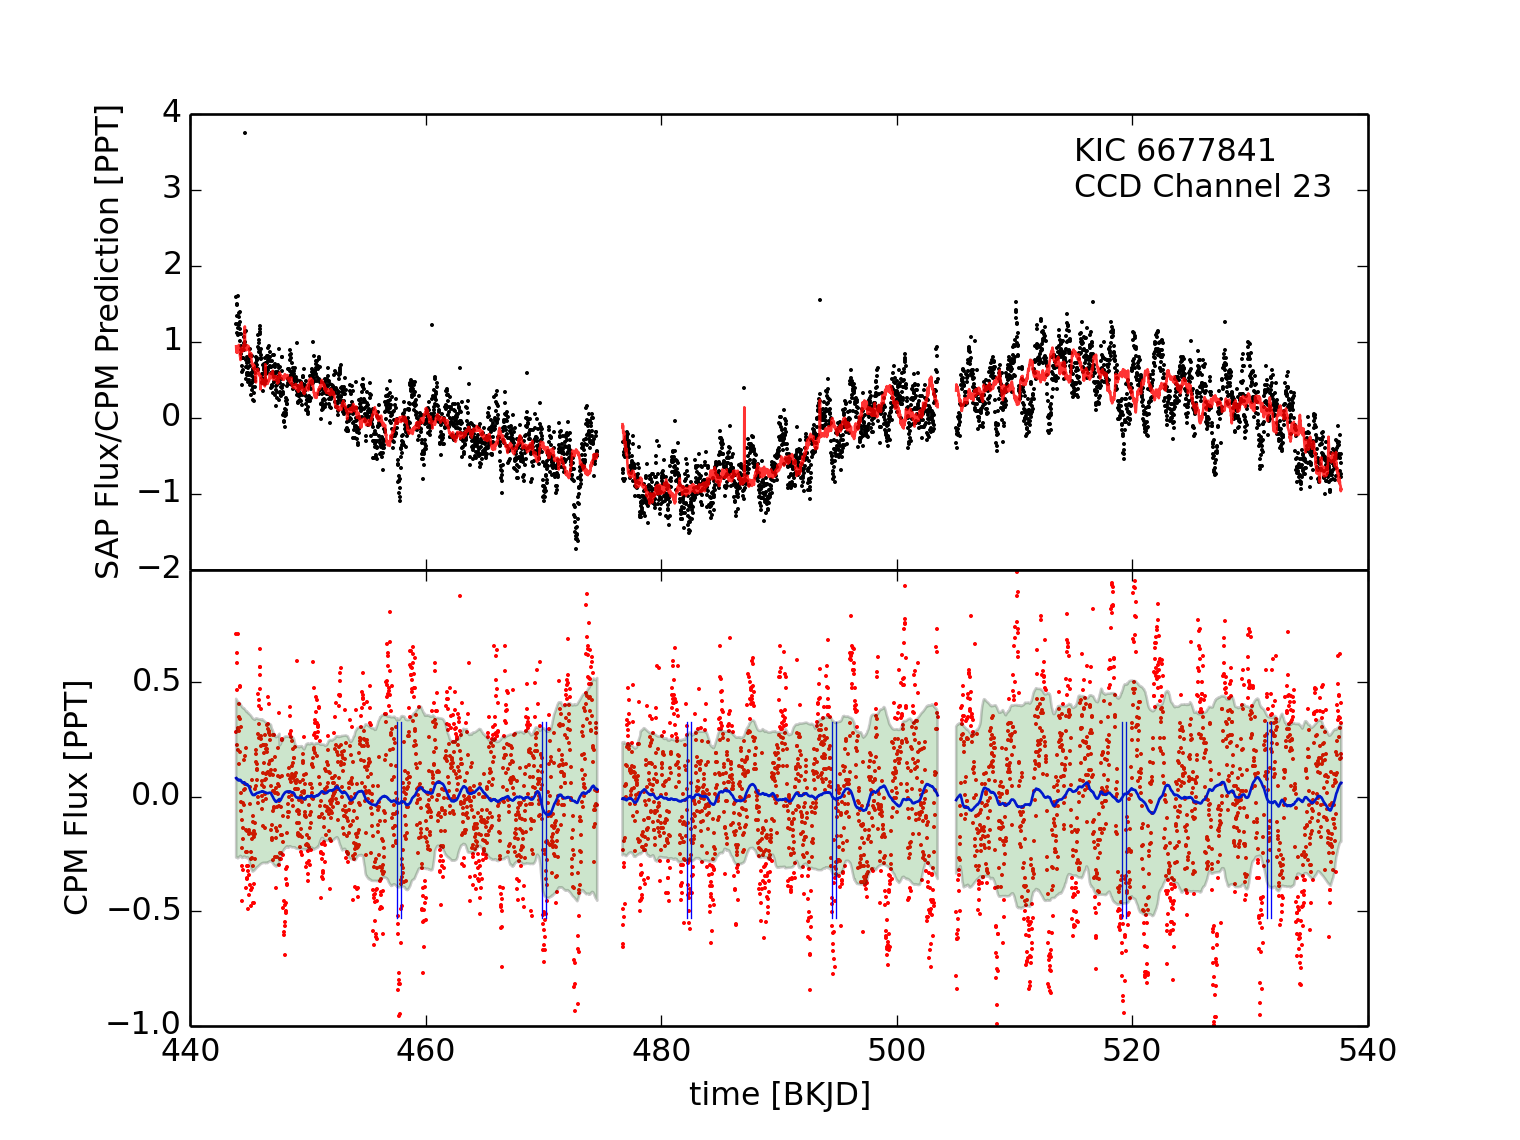
\includegraphics[width=\textwidth]{kic_6677841}
\end{subfigure}

\caption{\label{fluxes} Corrected fluxes using \name, for 12 example stars, spanning the main magnitude (brightness) range encountered. 
In first column plots,   we consider bright stars with magnitude from 9 to 10.5, second cloumn are stars with magnitude from 11 to 12.5,  
and the third column are faint stars with magnitude above 13. In the first two rows, we present some quiet stars. 
In all three panels, the top panel shows the SAP flux (black) and the CPM regression (red), i.e., our prediction of the star from other stars. 
The middle panel shows the CPM flux corrected using the regression, and the bottom shows the PDC flux. 
One can see that the CPM flux curve preserves the exoplanet transits (little downward spikes), 
while removing a substantial part of the variability present in the PDC flux. 
Both the bottom two rows present some variable stars with slow and fast variability. 
For the variable stars, we did not present the PDC comparison, since the PDC flux try to preserve intrinsic steller variability.}
\end{figure}


\begin{figure*}[htb]
\centering
\begin{subfigure}[htb]{0.33\columnwidth}
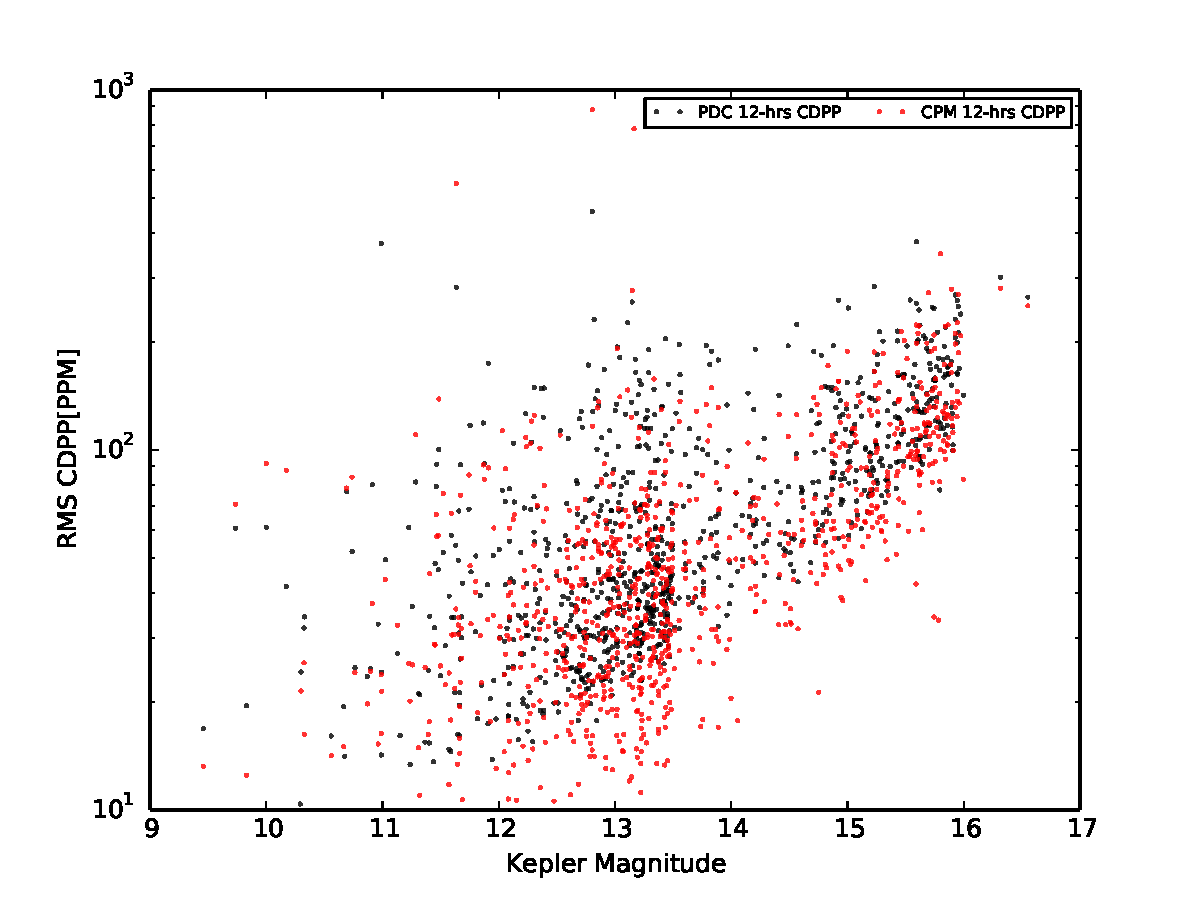
\includegraphics[width=\columnwidth]{pdc_cdpp12_r}
\caption{}
\end{subfigure}%
%\hfill
\begin{subfigure}[htb]{0.33\columnwidth}
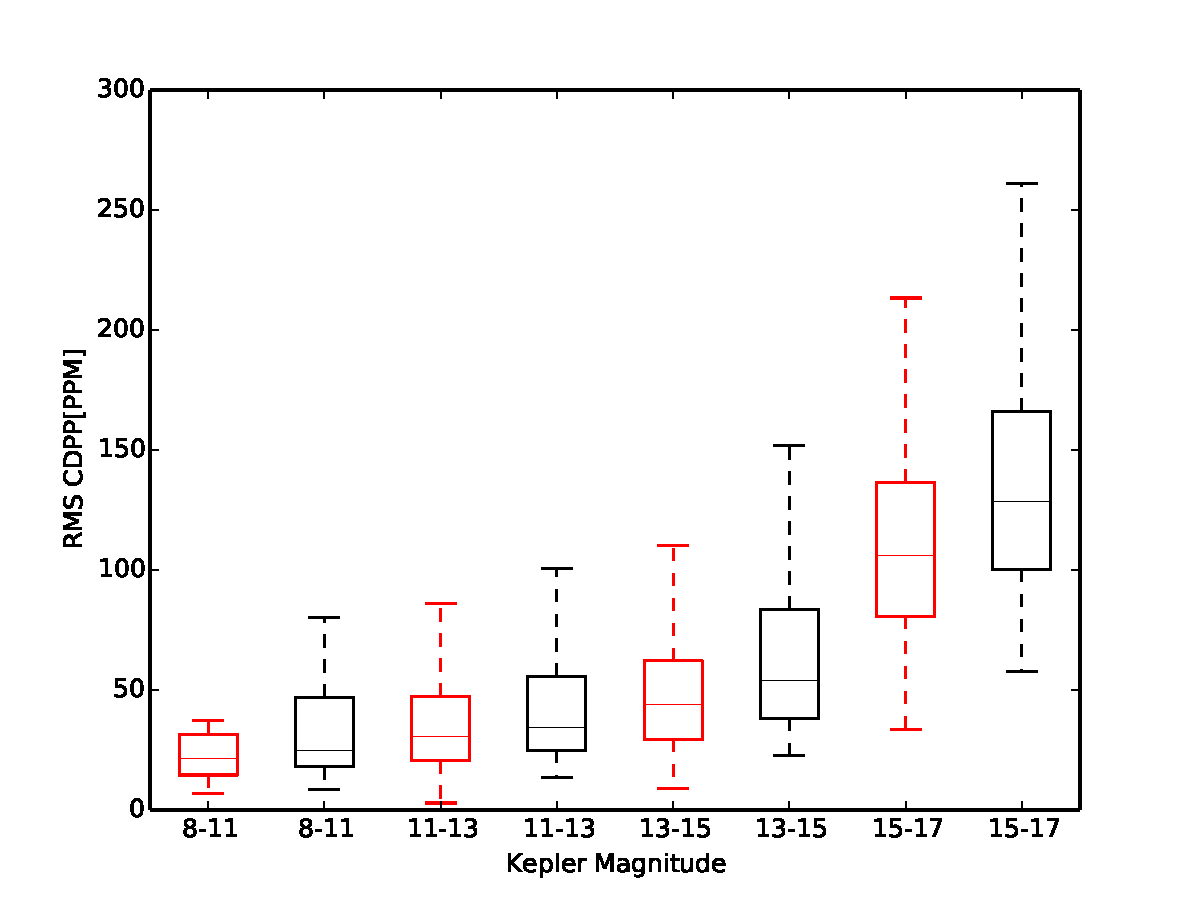
\includegraphics[width=\columnwidth]{boxplot_r}
\caption{}
\end{subfigure}%
%\hfill
\begin{subfigure}[htb]{0.33\columnwidth}
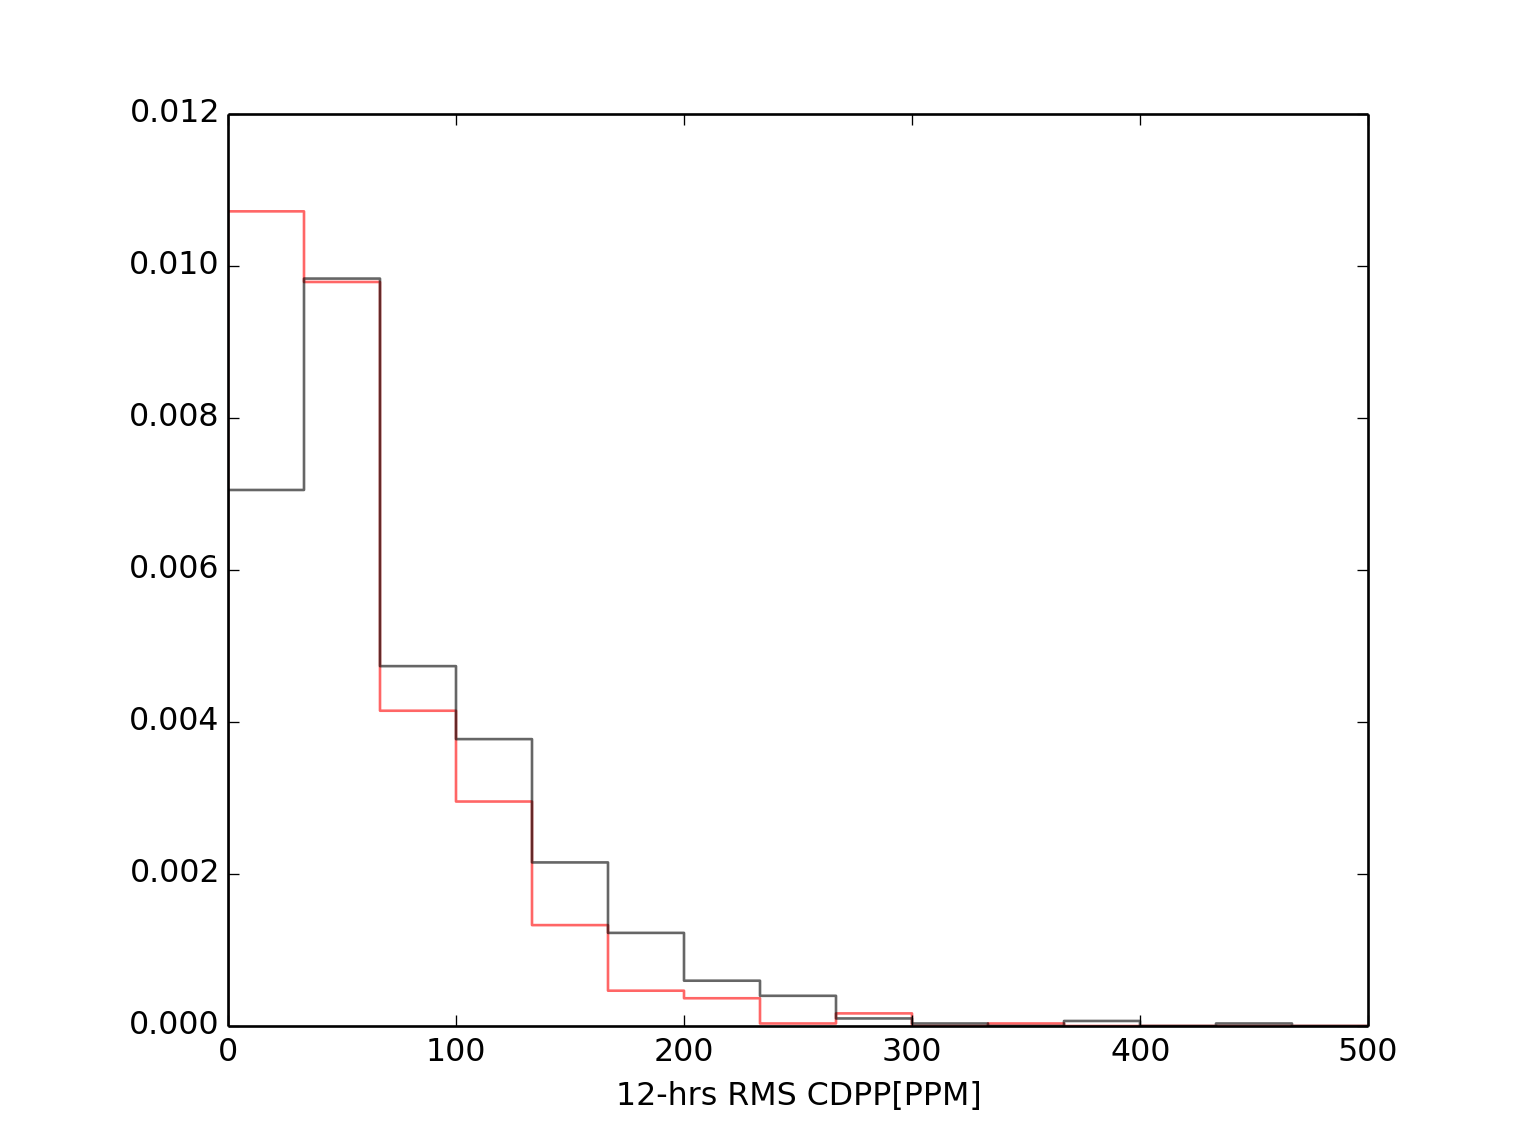
\includegraphics[width=\columnwidth]{pdc_cdpp12_hist_r100}
\caption{}
\end{subfigure}
\caption{\label{cdpp} Comparison of the proposed method (CPM) to the \Kepler\ Pre-search Data Conditioning (PDC) method 
in terms of Combined Differential Photometric Precision (CDPP) (see text). 
Plot (a) shows our performance (red) vs.\ the PDC performance in a scatter plot, as a function of star magnitude 
(note that larger magnitude means fainter stars, and smaller values of CDPP indicate a higher quality as measured by CDPP.  
Plot (b) bins the same dataset and shows box plots within each bin, indicating median, top quartile and bottom quartile. 
The red box corresponds to CPM, while the black box refers to PDC. Plot (c), finally, shows a histogram of CDPP values. 
Note that the red histogram has more mass towards the left, i.e., smaller values of CDPP, indicating that our method overall outperforms PDC, the Kepler ``gold standard.'' 
}
\end{figure*}

\clearpage

\section{Discussion}
We have presented a simple yet highly effective method that works in pixel-level 
based on the causal structure of the \Kepler\ data to calibrate the \Kepler\ light curves, 
which is intended to search exoplanets. 
However, based on our assumption of the causal structure of the \Kepler\ 
data, if we turn off the auto-regressive components and keep the predictors from other
stars working  in the \name, we should be able to still remove the systematics while
preserve the intrinsic stellar  variability, since there is no reason that these independent
stars can be used to predict the stellar variability of the target star. However, in fact, we
can not preserve the stellar variability just by turning off the auto-regressive 
components. One possible reason can be that, since our model is so flexible 
(thousands of parameters), in principle it can fit any functions. In this sense, we should 
run cross-validation with the auto-regressive components turned off and to find out how
many pixels from other stars we need to just remove systematics while preserve stellar
variability, but in fact we do not have a good criterion to check how well we preserve
stellar variability in cross-validation because we do not have enough knowledge of the 
true stellar variability. Thus for the time being, we just focus on producing well-
calibrated light curves for searching exoplanets, but in long term, we are looking
forward to find a method to preserve the stellar variability.

However, forget all the unsolved problems, we expect that our method will enable
astronomical discoveries at higher sensitivity on the existing \Kepler\ data as well as on
future missions.  As we know, \Kepler\ K2 data are suffering from the broken-down of
reaction wheels, which makes the satellite hard to control and introduce significant
systematics. Moreover, in 2017, NASA is planning the launch of another space 
telescope---TESS (Transiting Exoplanet Survey Satellite), which will perform an all-sky 
survey for small (earth-like) planets of nearby M stars. We think our method can be simply
extended for these project to help achieving higher precession and more scientific results. 


\acknowledgements
It is a pleasure to thank the whole \Kepler\ Team
  for designing, delivering, and operating a great facility,
  and for making all of the data public, in all its rawest forms, through the MAST interface.
We are also pleased to thank
  Ruth~Angus (Oxford),
  Tom~Barclay (Ames),
  Bekki~Dawson (Berkeley),
  Rob~Fergus (NYU),
  Stefan~Harmeling (Dusseldorf),
  Michael~Hirsch (UCL),
  Dustin~Lang (CMU),
  Benjamin~T.~Montet (Caltech),
  David~Schiminovich (Columbia),
  and
  Jake Vanderplas (UW)
for valuable discussions, input, encouragement, and advice.
This project was partially supported by
  NSF grant IIS-1124794,
  NASA grant NNX12AI50G.
  the Moore Foundation,
  and
  the Sloan Foundation.
This research made use of the NASA Astrophysics Data System.

\clearpage


\end{document}
